% Apresentação do trabalho de graduação

\documentclass{beamer}
\usepackage[brazil]{babel}
\usetheme{Warsaw} % tema do slide, o azul e preto no fundo
%\usetheme{Berlin}
%\usetheme{EastLansing}
%\usetheme{Luebeck}
%\usetheme{Copenhagen}
%\usetheme{Szeged}
%\usetheme{Singapore} %gostei
%\usetheme{AnnArbor}%nenhuma  cor fica legal
%\usetheme{CambridgeUS}%bom modelo
%\usetheme{Boadilla}%Muito bom
%\usetheme{Madrid}%excelente tema
%\usetheme{Boxes}
%\usetheme{Warsaw} % tema do slide, o azul e preto no fundo
%\usecolortheme{seahorse}
%\usecolortheme{beaver}
%\usecolortheme{albatross}
%\usecolortheme{crane}
\usecolortheme{dolphin}%bom esquema de cor
%\usecolortheme{dove}
%\usecolortheme{fly}
%\usecolortheme{lily}
%\usecolortheme{orchid}%ótimo com Cambridge
%\usecolortheme{rose}
%\usecolortheme{seagull}
%\usecolortheme{sidebartab}
%\usecolortheme{structure}
%\usecolortheme{whale}
%\usecolortheme{wolverine}
\usepackage{hyperref}
\usepackage{graphicx}
\usepackage{ragged2e}
\usepackage{latexsym}
%\usepackage[latin1]{inputenc}
\usepackage[utf8]{inputenc} % esse serve pra digitar com acento normal
\usepackage{amsmath}
\usepackage{amsfonts}
\usepackage{amssymb}
\usepackage{multicol}

\usepackage{listings}
\usepackage{courier}
\usepackage{graphics}
\usepackage{color} 
\usepackage{subcaption}


% ---------------------
% Definição da listagem de código-fonte
% ---------------------
\lstset{
         basicstyle=\footnotesize\ttfamily, % Standardschrift
         %numbers=left,               % Ort der Zeilennummern
         numberstyle=\tiny,          % Stil der Zeilennummern
         %stepnumber=2,               % Abstand zwischen den Zeilennummern
         numbersep=5pt,              % Abstand der Nummern zum Text
         tabsize=2,                  % Groesse von Tabs
         extendedchars=true,         %
         breaklines=true,            % Zeilen werden Umgebrochen
         keywordstyle=\color{red},
    		frame=b,         
  %       keywordstyle=[1]\textbf,    % Stil der Keywords
 %        keywordstyle=[2]\textbf,    %
  %       keywordstyle=[3]\textbf,    %
 %        keywordstyle=[4]\textbf,   \sqrt{\sqrt{}} %
         stringstyle=\color{white}\ttfamily, % Farbe der String
         showspaces=false,           % Leerzeichen anzeigen ?
         showtabs=false,             % Tabs anzeigen ?
         xleftmargin=17pt,
         framexleftmargin=17pt,
         framexrightmargin=5pt,
         framexbottommargin=4pt,
         %backgroundcolor=\color{lightgray},
         showstringspaces=false      % Leerzeichen in Strings anzeigen ?        
 }
 \lstloadlanguages{
         C++
 }

\renewcommand\lstlistingname{Código}
\renewcommand\lstlistlistingname{Códigos}

\useoutertheme[subsection=false,shadow=default]{miniframes}
\useinnertheme{default}
\setbeamertemplate{footline}{}
%\beamertemplatenavegationsymbolsempty{}

%\setlength{\parindent}{-10cm} 

\title[Defesa]{Implementação de Suporte a Texturas 3D para Renderização de
Volumes no Blender}
\author[Rafael Campos]{Rafael Cerqueira de Campos \\ Orientador: Prof. Dr. Mario Augusto de Souza Liziér}
\institute[DC - UFSCAR]{Graduação em Engenharia de Computação - UFSCar}
\date{\today}
\thispagestyle{empty}
\subject{alguma coisa}

%%Define o caminho das figuras, válido somente para o comando \includegraphics
\graphicspath{{images/}}

\begin{document}


%Primeira página da apresentação
\frame{\titlepage}

\AtBeginSubsection[]

%%%%%%%%%%%%%%%%%%%%%%%%%%%%%%%%%%%%%%%%%%%%%%%%%%%%%%
%Sum\'ario
\begin{frame}[allowframebreaks]
\tableofcontents
\end{frame}
%%%%%%%%%%%%%%%%%%%%%%%%%%%%%%%%%%%%%%%%%%%%%%%%%%%%%%

%%%%%%% Primeiro Slide %%%%%%%%%%%%%%%%%%%%%%%%%%%%%%%%%%%%%%%%%
\section{Motivação}
\subsection{}

\begin{frame}

\frametitle{Motivação}
\begin{itemize}
\item Projeto
\item Funcionalidade
\item Aplicação
\item Escolha de biblioteca
\end{itemize}

\end{frame}

%%%%%%%%%%%%%%%%%%%%%%%%%%%%%%%%%%%%%%%%%%%%%%%%%%%%%%%%%   

%%
\begin{frame}

\begin{multicols}{2}
\frametitle{Projeto}
\begin{itemize}
\item Projeto pessoal
\item Google Summer of Code
\begin{itemize}
    \item Blender Foundation
    \item Proposta de Trabalho
\end{itemize}

\item Metodologia de Desenvolvimento
\begin{itemize}
\item Ambiente: CMake + Clang; Subversion
\item Discussões abertas
\item Relatórios, Reuniões e Documentação
\end{itemize}
\end{itemize}
\begin{center}

\includegraphics[width=5cm]{gsoc}
\end{center}
\end{multicols}



\end{frame}
%%%%%%%%%%%%%%%%%%%%%%%%%%%%%%%%%%%%%%%%%%%%%%%%%%%%%%%%%   
%%%%%%%%%%%%%%%%%%%%%%%%%%%%%%%%%%%%%%%%%%%%%%%%%%%%%%%%%	

%%
\begin{frame}

\begin{figure}[t]
\center
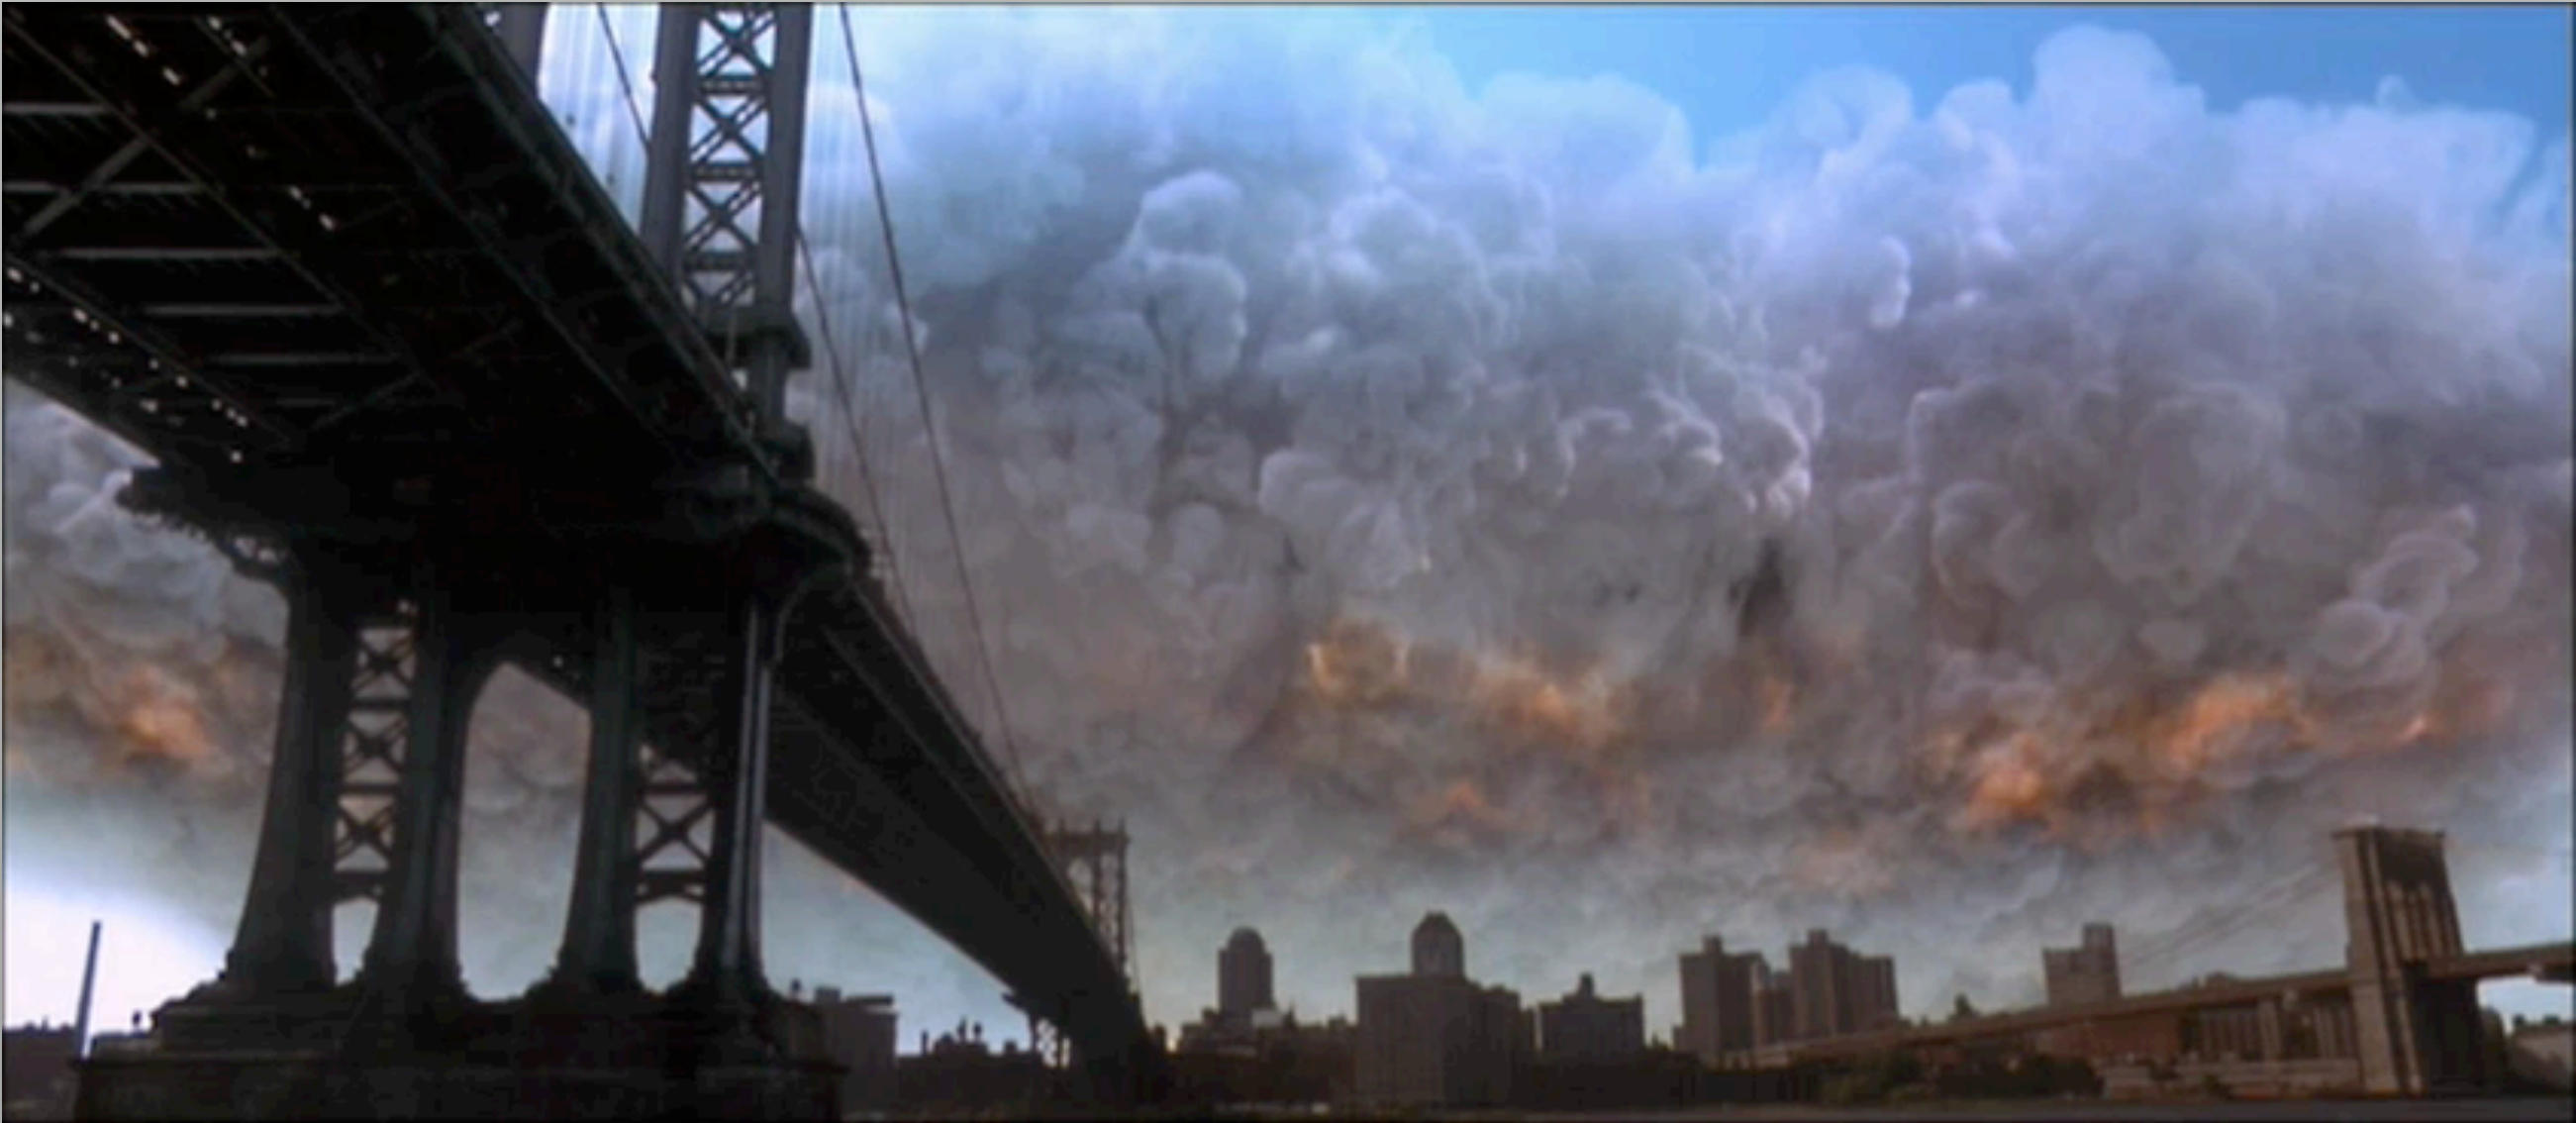
\includegraphics[width=10cm]{independenceDay}
\caption*{\tiny © 1996 Twentieth Century Fox and Centropolis Entertainment. All 
rights reserved.}
\end{figure}

\frametitle{Funcionalidade}
\begin{itemize}
\item Nuvens, névoa, fogo, tempestades de areia...
\item Simulação x Modelagem
\end{itemize}

\end{frame}
%%%%%%%%%%%%%%%%%%%%%%%%%%%%%%%%%%%%%%%%%%%%%%%%%%%%%%%%%   
%%


%%
\begin{frame}

\begin{figure}[t]
\center
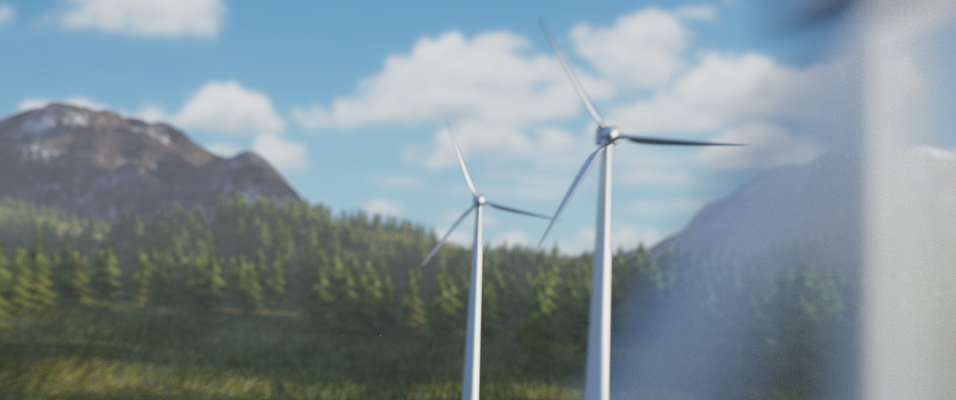
\includegraphics[width=9cm]{cyclesHeader}
\caption*{\tiny Fonte: http://cgcookie.com/blender/2013/03/11/creating-mist-blender-cycles-z-depth/}
\end{figure}

\frametitle{Aplicação}
Cycles
\begin{itemize}
\item Traçador de raios
\item Sem suporte a renderização de volumes
\end{itemize}

\end{frame}
%%%%%%%%%%%%%%%%%%%%%%%%%%%%%%%%%%%%%%%%%%%%%%%%%%%%%%%%% 
%%
\begin{frame}

\frametitle{Escolha de biblioteca}
Considerações
\begin{itemize}
\item Aplicação: animação x jogos
\item Representação de volumes
\item Aceitação e adoção
\end{itemize}

\begin{figure}[b]
        \centering
        \begin{subfigure}{0.3\textwidth}
                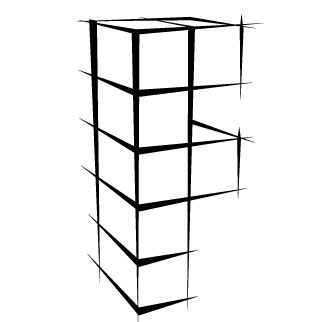
\includegraphics[width=\textwidth]{field3d}
                \caption*{Field3D}
        \end{subfigure}%
        ~ %add desired spacing between images, e. g. ~, \quad, \qquad etc.
          %(or a blank line to force the subfigure onto a new line)
        \begin{subfigure}{0.3\textwidth}
                
\includegraphics[width=\textwidth]{openvdbLogo}  
        \end{subfigure}
        ~ %add desired spacing between images, e. g. ~, \quad, \qquad etc.
          %(or a blank line to force the subfigure onto a new line
        \begin{subfigure}{0.3\textwidth}
                
\includegraphics[width=\textwidth]{gigavoxelsLogo}
        \end{subfigure}    
\end{figure}

\end{frame}
%%%%%%%%%%%%%%%%%%%%%%%%%%%%%%%%%%%%%%%%%%%%%%%%%%%%%%%%% 

%%%%%%% n-th Slide %%%%%%%%%%%%%%%%%%%%%%%%%%%%%%%%%%%%%%%%%
\section{Blender}
\subsection{}
\begin{frame}

\frametitle{Software: Blender}

\begin{figure}[!htb]
\center
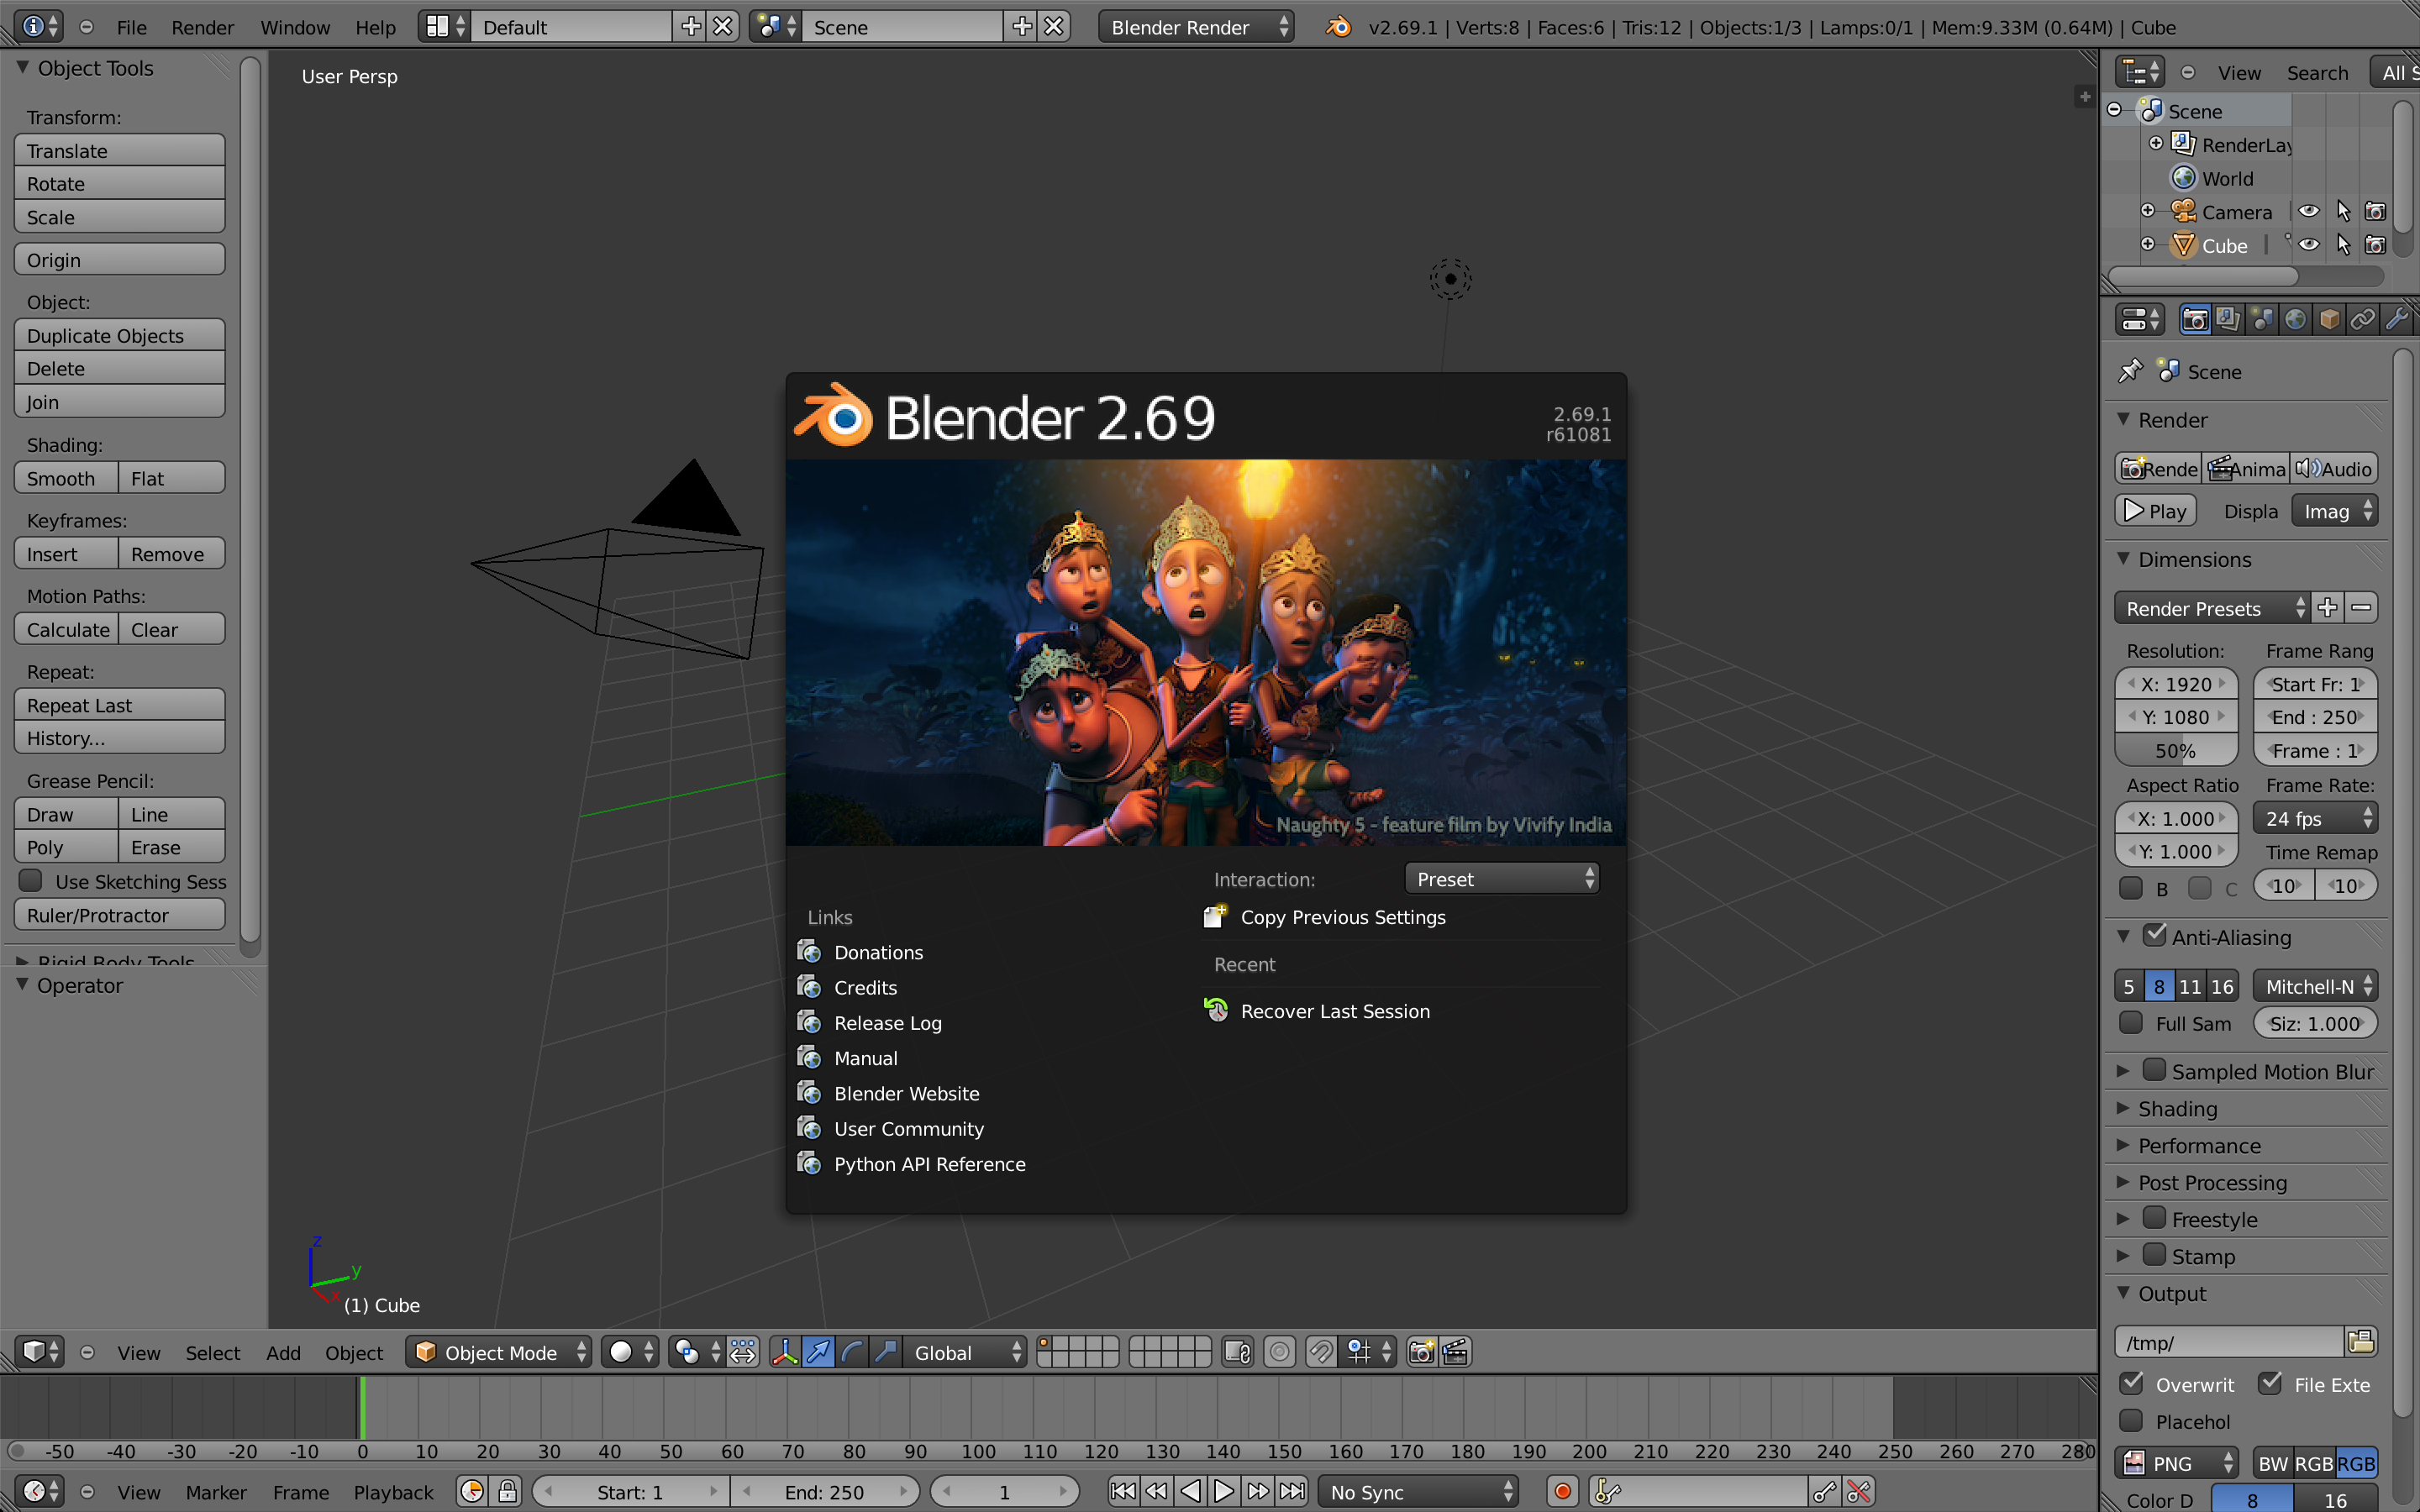
\includegraphics[width=10cm]{blender_gui}
\end{figure}


\end{frame}
%%%%%%%%%%%%%%%%%%%%%%%%%%%%%%%%%%%%%%%%%%%%%%%%%%%%%%%%%	
%%%%%%% n-th Slide %%%%%%%%%%%%%%%%%%%%%%%%%%%%%%%%%%%%%%%%%
\begin{frame}

\frametitle{Renderização no Blender}
\begin{itemize}
\item Blender Internal Render
    \begin{itemize}
        \item Amplamente testado
        \item Suporta renderização de volumes
        \item Fraco desempenho em simulação cáustica: vidros, metais
        \item Comportamento não é realista
    \end{itemize}
\item Cycles Render
    \begin{itemize}
        \item Algoritmo traçador de raios
        \item Simulação cáustica é consequência do funcionamento
        \item Fisicamente plausível
    \end{itemize}
\item Blender Game Engine
\begin{itemize}
    \item Usado exclusivamente para jogos
    \item O resultado é um executável
 \end{itemize}
\end{itemize}

\end{frame}

\begin{frame}

\frametitle{Comparação entre \emph{engines}}

\begin{figure}[!htb]
        \centering
        \begin{subfigure}{0.5\textwidth}
                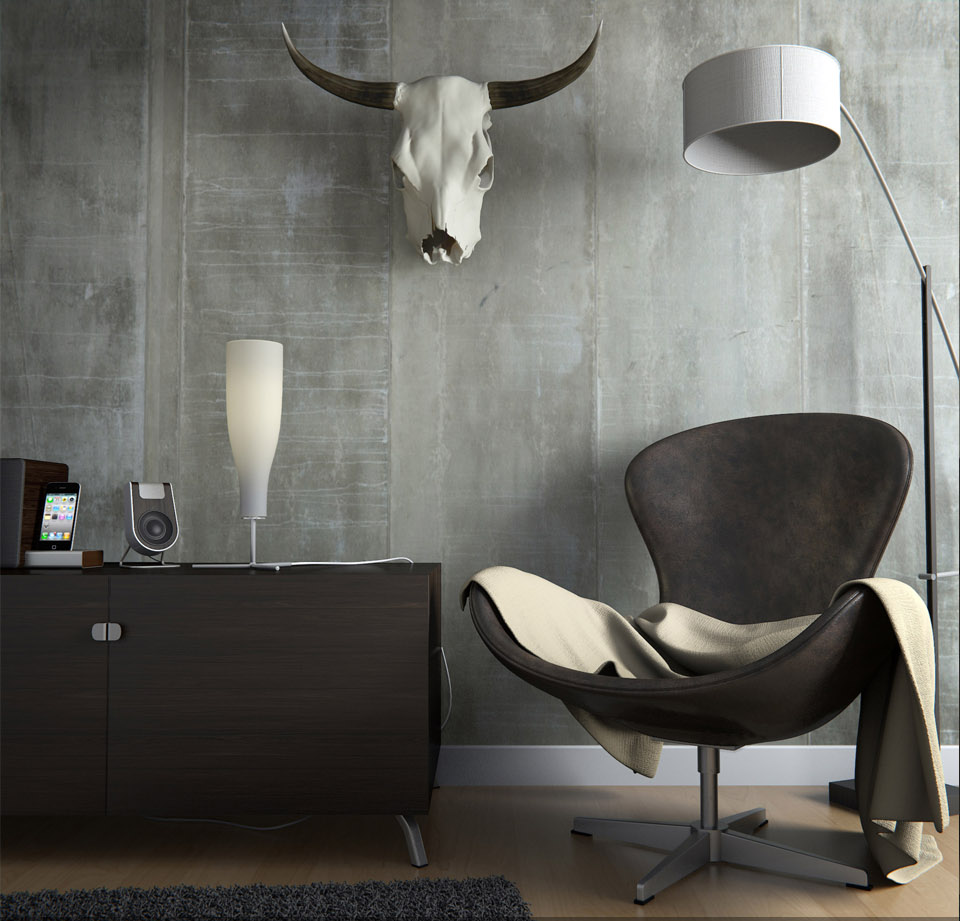
\includegraphics[width=\textwidth]{blenderInternalRender}
                \caption*{Blender Internal}
        \end{subfigure}%
        ~ %add desired spacing between images, e. g. ~, \quad, \qquad etc.
          %(or a blank line to force the subfigure onto a new line)
        \begin{subfigure}{0.5\textwidth}
                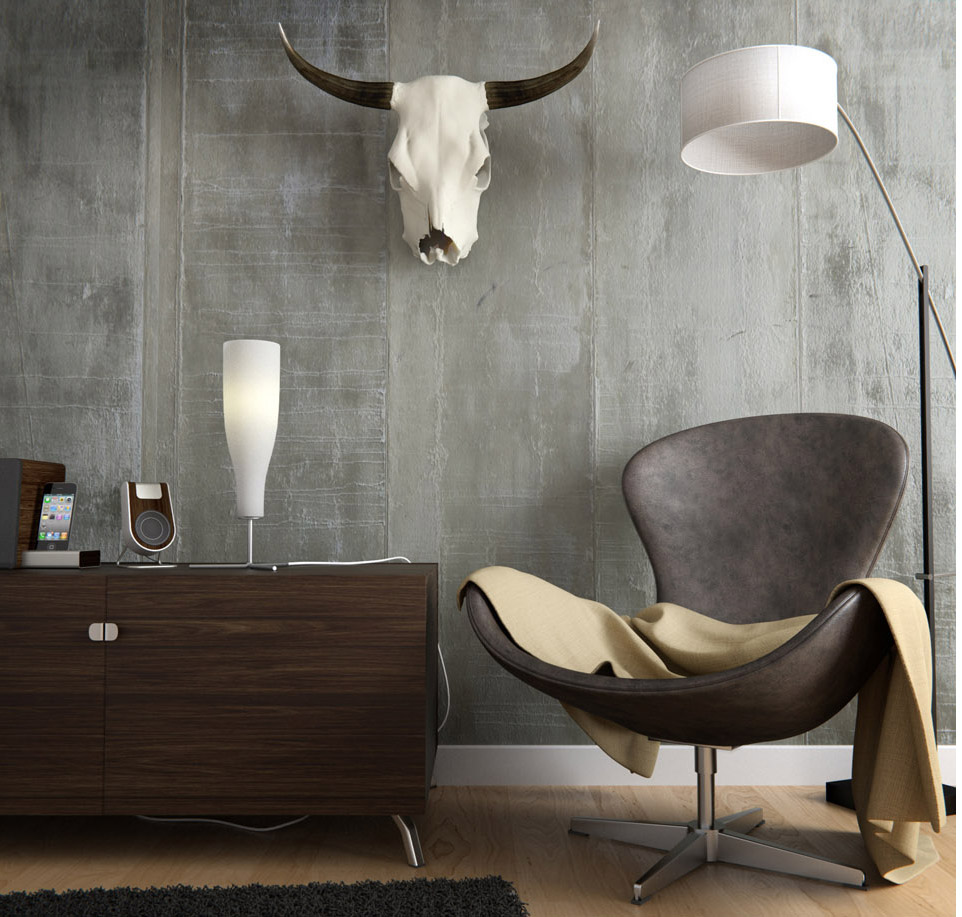
\includegraphics[width=\textwidth]{cyclesRender} 
                \caption*{Cycles} 
        \end{subfigure}
        \caption*{\tiny Fonte: http://www.blendernation.com/2012/06/16/bi-vs-cycles-vs-yafray-an-artists-observation/ }
\end{figure}

\end{frame}


\begin{frame}

\frametitle{Cycles}
\begin{itemize}
\item Baseado em nós

\item Comportamento configurável por {\it scripts}
\end{itemize}


\end{frame}

%%%%%%%%

\begin{frame}

\frametitle{Cycles: Configuração por nós}

\begin{figure}[!htb]
\center
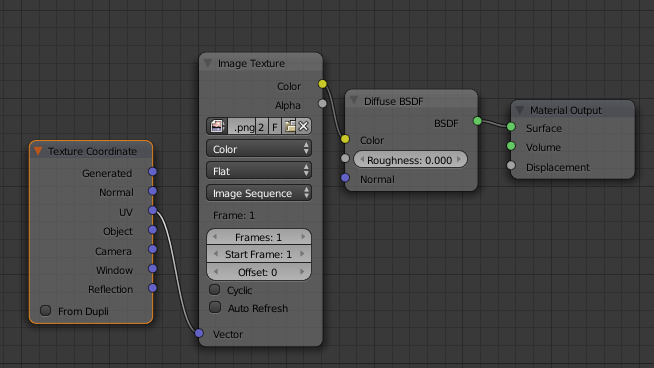
\includegraphics[width=9cm]{Cycles_nodes}
\caption{Rede de nós configurando o uso de uma sequência de imagens como textura para uma superfície.}
\end{figure}

\end{frame}
%%%%%%%%

%%%%%%%%
\begin{frame}

\frametitle{Cycles: Configuração por nós}

\begin{figure}[!htb]
\center
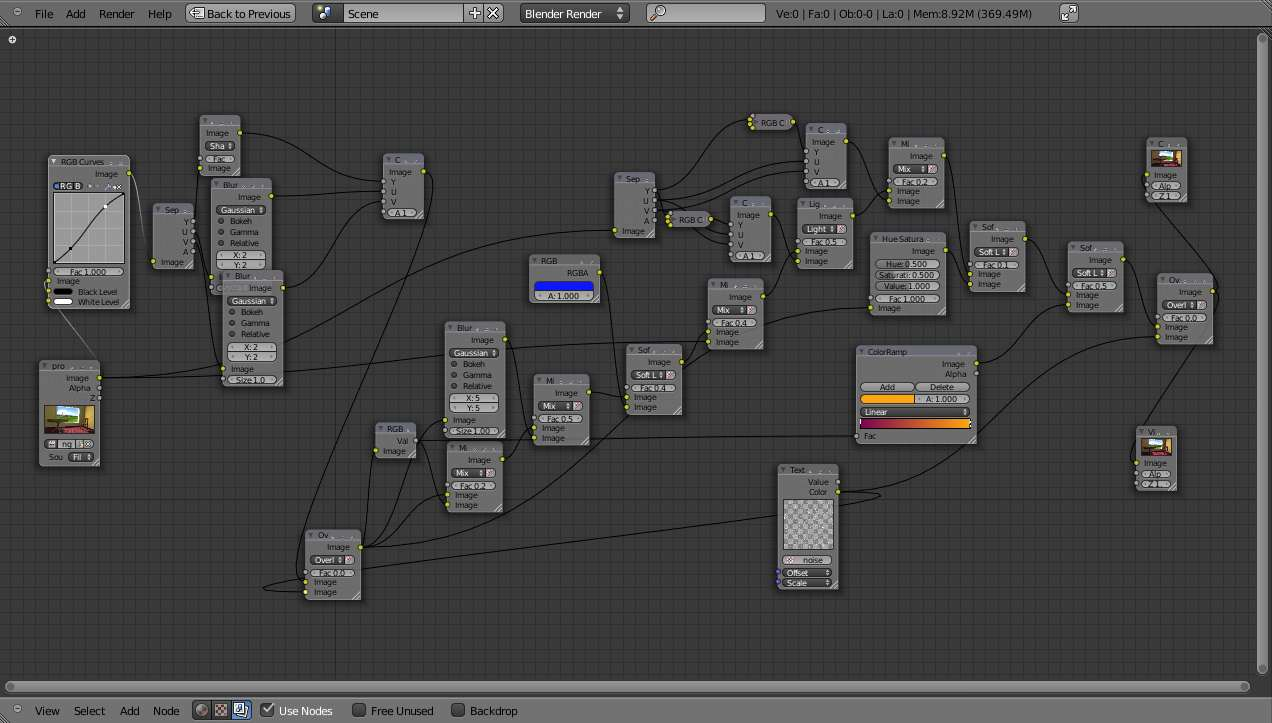
\includegraphics[width=10cm]{film_lookNodeNetwork}
\caption{Rede de nós para emular a aparência de impressão sobre filme.}
\end{figure}

\end{frame}
%%%%%%%%

\subsection{}
\begin{frame}
\frametitle{Open Shading Language}
\begin{itemize}
\item Especificação de uma linguagem
\item \texttt{oslc} \\ Compilador de arquivos OSL para \emph{bytecode}
\item \texttt{liboslexec} \\ Compilação {\it JIT} com LLVM para transformar o \emph{bytecode} do {\it shaders} em instruções x86
\item Biblioteca de shaders
\end{itemize}
\end{frame}


%%%%%%%%
\begin{frame}

\frametitle{Texturas Tridimensionais}

\begin{figure}[!htb]
\center
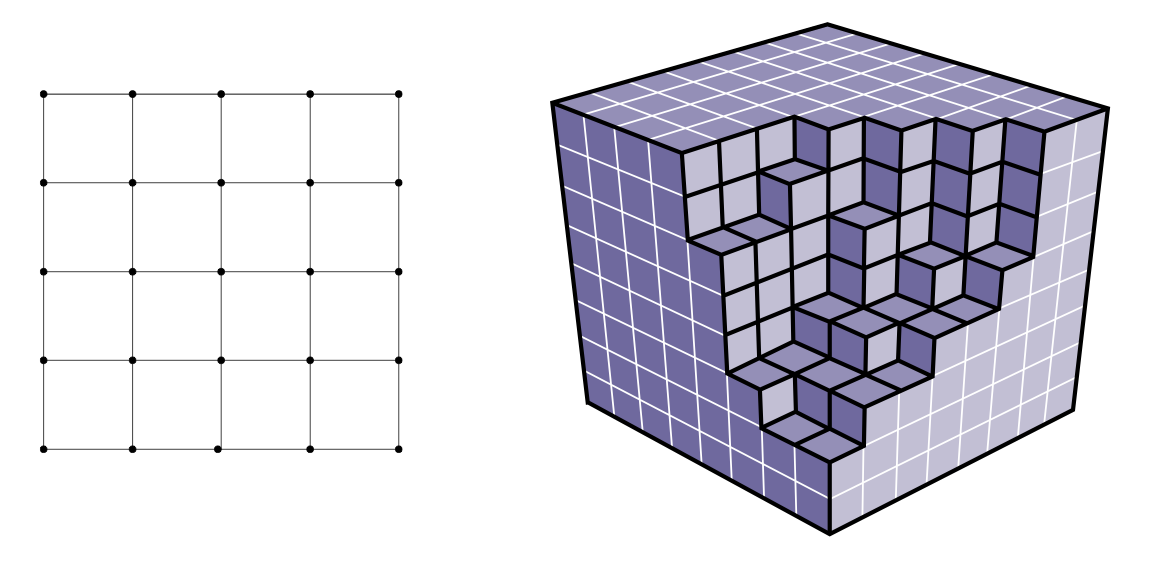
\includegraphics[width=7cm]{grid_example}
\caption*{\tiny Fonte: Wrenninge, Magnus (2013-01-31). Production Volume Rendering: Design and Implementation (Page 47). A K Peters/CRC Press. Kindle Edition.}
\end{figure}

\end{frame}
%%%%%%%%

\begin{frame}

\frametitle{Texturas Tridimensionais}

\lstinputlisting[caption={Consulta ao valor de ponto flutuante no voxel de coordenadas (1, 2, 3)}]{../sourceCode/vdb_coordinates.cpp}

\end{frame}
%%%%%%%%

\begin{frame}

\frametitle{Volumes Esparsos}

\begin{figure}[!htb]
\center
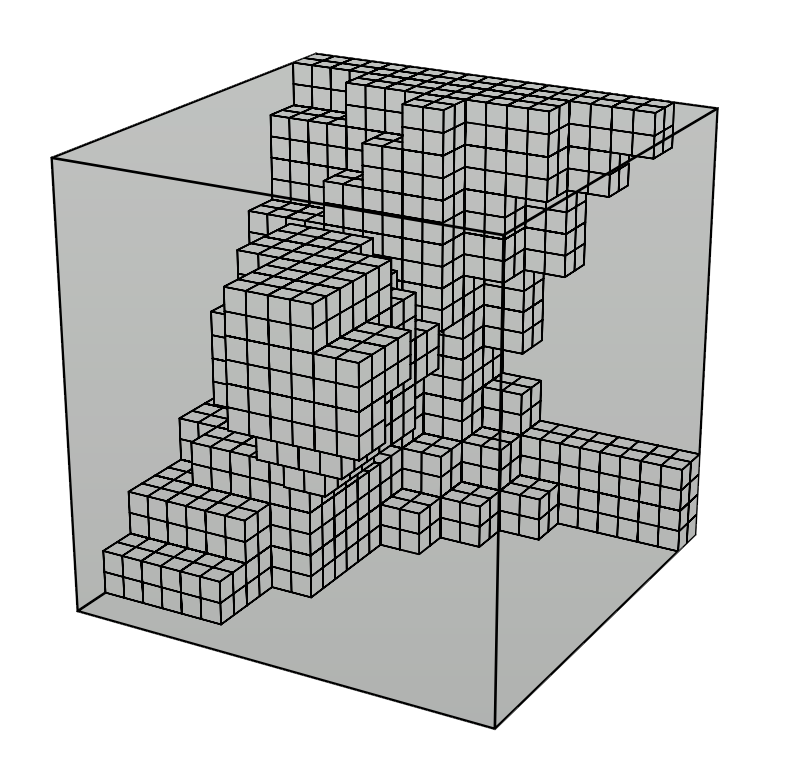
\includegraphics[width=7cm]{sparse}  
\caption*{\tiny Fonte: Wrenninge, Magnus (2013-01-31). Production Volume Rendering: Design and Implementation (Page 52). A K Peters/CRC Press. Kindle Edition.}
\end{figure}

\end{frame}



%%%%%%%%%%%%%%%%%%%%%%%%%%%%%%%%%%%%%%%%%%%%%%%%%%%%%%%%%
%%%%%%% n-th Slide %%%%%%%%%%%%%%%%%%%%%%%%%%%%%%%%%%%%%%%%%
\section{OpenVDB}
\subsection{}
\begin{frame}

\frametitle{OpenVDB: Motivação}

\begin{figure}[!htb]
\center
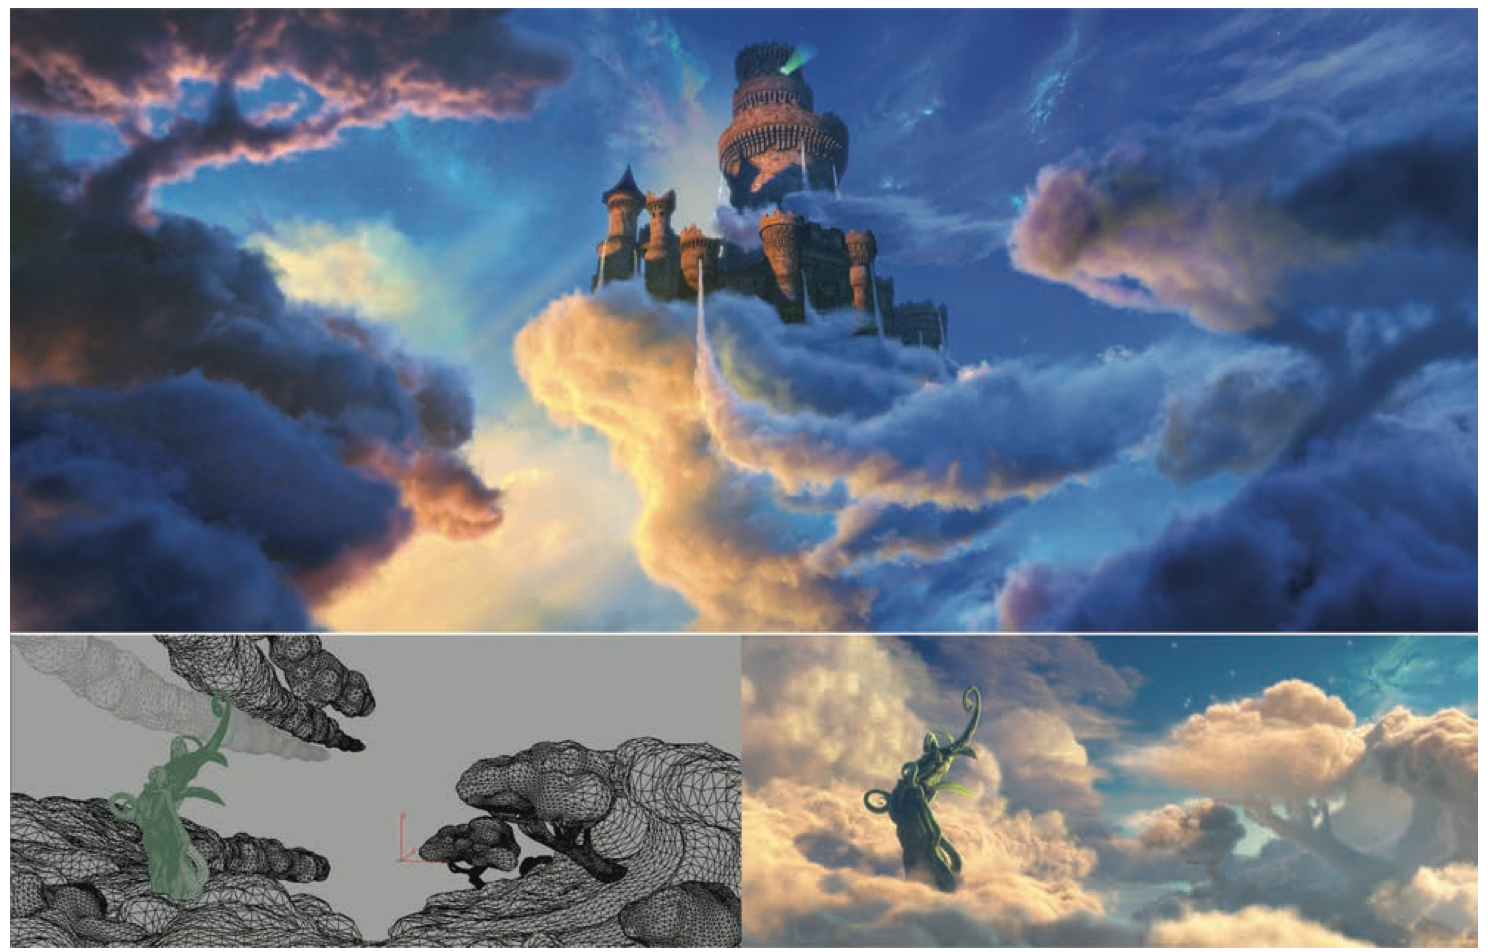
\includegraphics[width=10cm]{puss}
\caption*{\tiny Fonte: Museth, K. 2013. VDB: High-resolution sparse volumes with dynamic topology. ACM Trans. Graph. 32, 3, Article 27 (June 2013). Page 2.}
\end{figure}

\end{frame}
%%%%%%%%%%%%%%%%%%%%%%%%%%%%%%%%%%%%%%%%%%%%%%%%%%%%%%%%%	

%%%%%%% n-th Slide %%%%%%%%%%%%%%%%%%%%%%%%%%%%%%%%%%%%%%%%%
\begin{frame}

\frametitle{Características}

\begin{itemize}
\item Dinâmico
\item Uso eficiente de memória
\item Topologia genérica
\item Acesso rápido aleatório e sequencial
\item Virtualmente infinito
\item Resolução Adaptativa
\end{itemize}

\end{frame}
%%%%%%%%%%%%%%%%%%%%%%%%%%%%%%%%%%%%%%%%%%%%%%%%%%%%%%%%%	

%%%%%%% n-th Slide %%%%%%%%%%%%%%%%%%%%%%%%%%%%%%%%%%%%%%%%%

\begin{frame}

\frametitle{Terminologia}

\begin{itemize}
\item \emph{Voxel}
\begin{itemize}
\item Menor unidade de volume endereçável na estrutura de dados
\item Na árvore, é localizado nas folhas
\end{itemize}
\item Valor Intermediário
\begin{itemize}
\item Valor constante aplicável a uma região do domínio
\item Na árvore, está nos nós intermediários, entre raiz e folhas
\end{itemize}
\item Estado Ativo
\begin{itemize}
\item Todos os valores (\emph{voxels} e valores intermediários) possuem um estado binário
\item Significado é dado pela aplicação
\end{itemize}
\end{itemize}

\end{frame}
%%%%%%%%%%%%%%%%%%%%%%%%%%%%%%%%%%%%%%%%%%%%%%%%%%%%%%%%%	

%%%%%%% n-th Slide %%%%%%%%%%%%%%%%%%%%%%%%%%%%%%%%%%%%%%%%%
\begin{frame}

\frametitle{Exemplo de um volume: modelo e representação de dados}

\begin{figure}[!htb]
\center
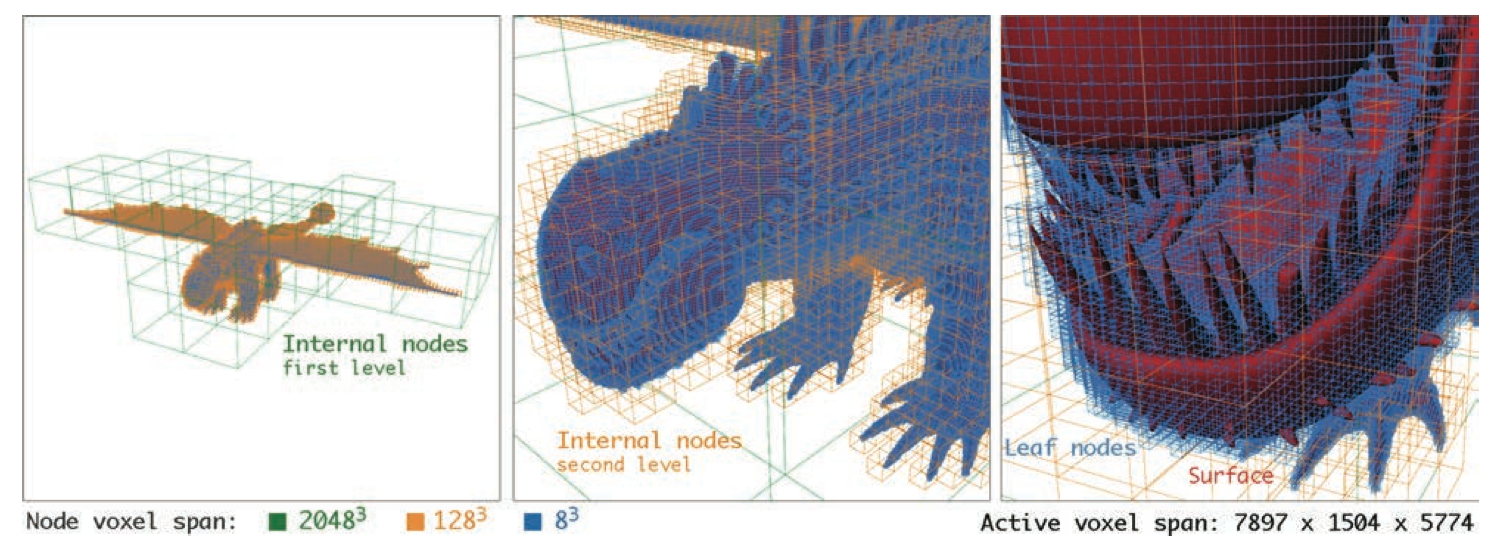
\includegraphics[width=10cm]{dragon}  
\caption*{\tiny Fonte: Museth, K. 2013. VDB: High-resolution sparse volumes with dynamic topology. ACM Trans. Graph. 32, 3, Article 27 (June 2013). Page 6.}
\end{figure}

\end{frame}
%%%%%%%%%%%%%%%%%%%%%%%%%%%%%%%%%%%%%%%%%%%%%%%%%%%%%%%%%
%%%%%%% n-th Slide %%%%%%%%%%%%%%%%%%%%%%%%%%%%%%%%%%%%%%%%%

\begin{frame}

\frametitle{Acesso aos Dados}

\begin{itemize}
\item Acesso Sequencial
\begin{itemize}
\item Fundamental para simulações
\item Acessa os elementos pela disposição física na memória
\item Operações de E/S com compressão específica para o formato
\end{itemize}
\item Acesso Aleatório
\begin{itemize}
\item Acesso por coordenadas: \texttt{getValue(x,y,z)}
\item Coerência espacial
\end{itemize}
\item Acesso por Estêncil
\begin{itemize}
\item Fundamental para diferenciação finita, filtragem e interpolação
\item Normalmente combinada com acesso sequencial ou aleatório
\end{itemize}
\end{itemize}

\end{frame}
%%%%%%%%%%%%%%%%%%%%%%%%%%%%%%%%%%%%%%%%%%%%%%%%%%%%%%%%%

%%%%%%% n-th Slide %%%%%%%%%%%%%%%%%%%%%%%%%%%%%%%%%%%%%%%%%
\subsection{}
\begin{frame}

\frametitle{Estrutura de Dados}

\begin{figure}[!htb]
\center
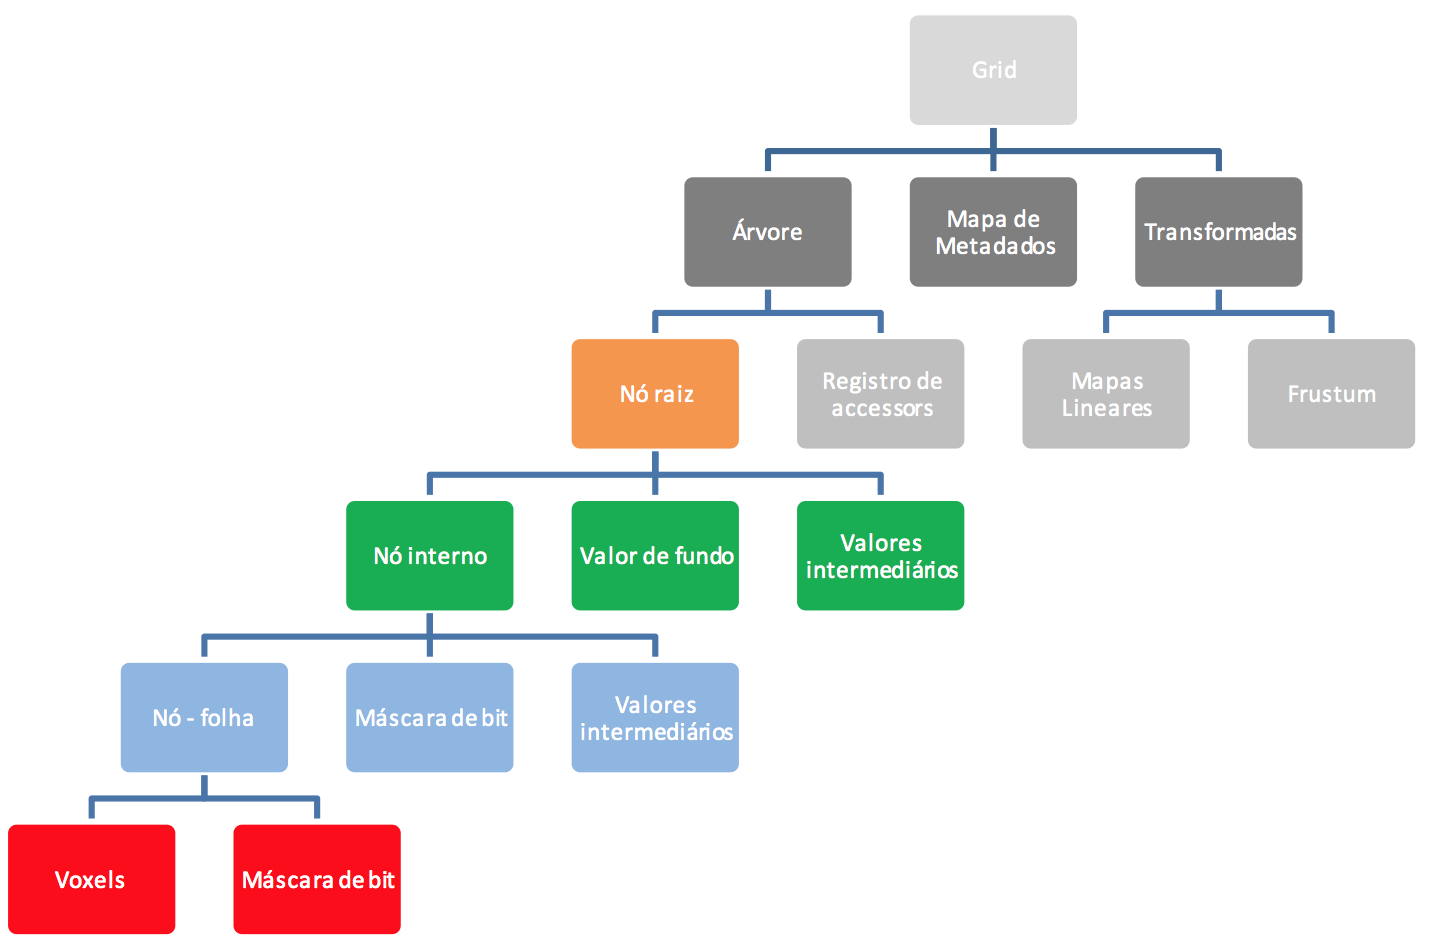
\includegraphics[width=10cm]{tree_structure}  
\end{figure}

\end{frame}
%%%%%%%%%%%%%%%%%%%%%%%%%%%%%%%%%%%%%%%%%%%%%%%%%%%%%%%%%
%%%%%%% n-th Slide %%%%%%%%%%%%%%%%%%%%%%%%%%%%%%%%%%%%%%%%%

\begin{frame}

\frametitle{Estrutura de Dados}

\begin{figure}[!htb]
\center
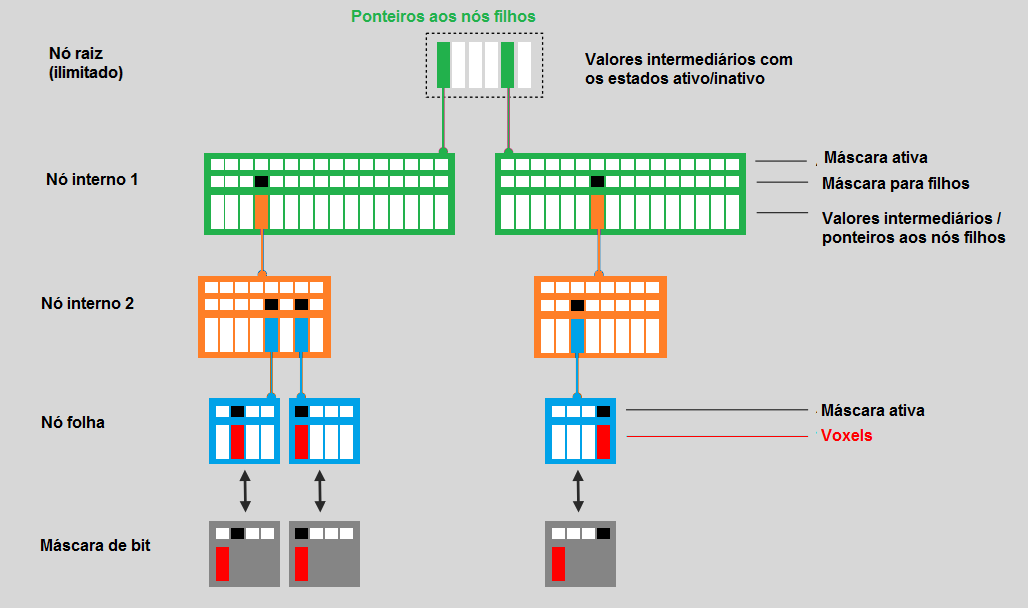
\includegraphics[width=10cm]{tree_inverted}  
\end{figure}

\end{frame}
%%%%%%%%%%%%%%%%%%%%%%%%%%%%%%%%%%%%%%%%%%%%%%%%%%%%%%%%%

%%%%%%% n-th Slide %%%%%%%%%%%%%%%%%%%%%%%%%%%%%%%%%%%%%%%%%

\begin{frame}

\frametitle{Dados Esparsos e Eficiência de Acesso}

\begin{itemize}
\item Eficiência no uso de memória
\begin{itemize}
\item Árvore hierárquica e esparsa
\item Memória alocada no momento de inserção
\item Operações de E/S com compressão específica para o formato
\end{itemize}
\item Eficiência Computacional
\begin{itemize}
\item Algoritmos hierárquicos
\item Cálculos esparsos
\item Metaprogramação com \texttt{templates} C++
\item Suporte a paralelismo, operações {\it bit} a {\it bit} e \emph{SIMD}
\end{itemize}
\end{itemize}

\end{frame}
%%%%%%%%%%%%%%%%%%%%%%%%%%%%%%%%%%%%%%%%%%%%%%%%%%%%%%%%%

%%%%%%% n-th Slide %%%%%%%%%%%%%%%%%%%%%%%%%%%%%%%%%%%%%%%%%
\section{Resultados}
\subsection{}

\begin{frame}

\frametitle{Resultados}

\begin{figure}[!htb]
\center
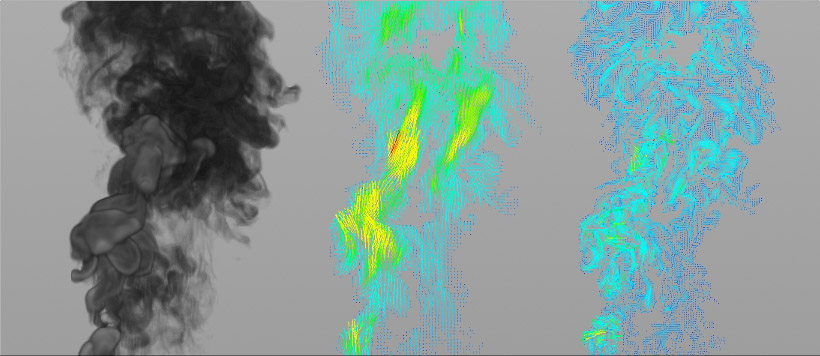
\includegraphics[width=6cm]{example_vector}  
\end{figure}

\begin{figure}[H]
        \centering
        \begin{subfigure}{0.3\textwidth}
                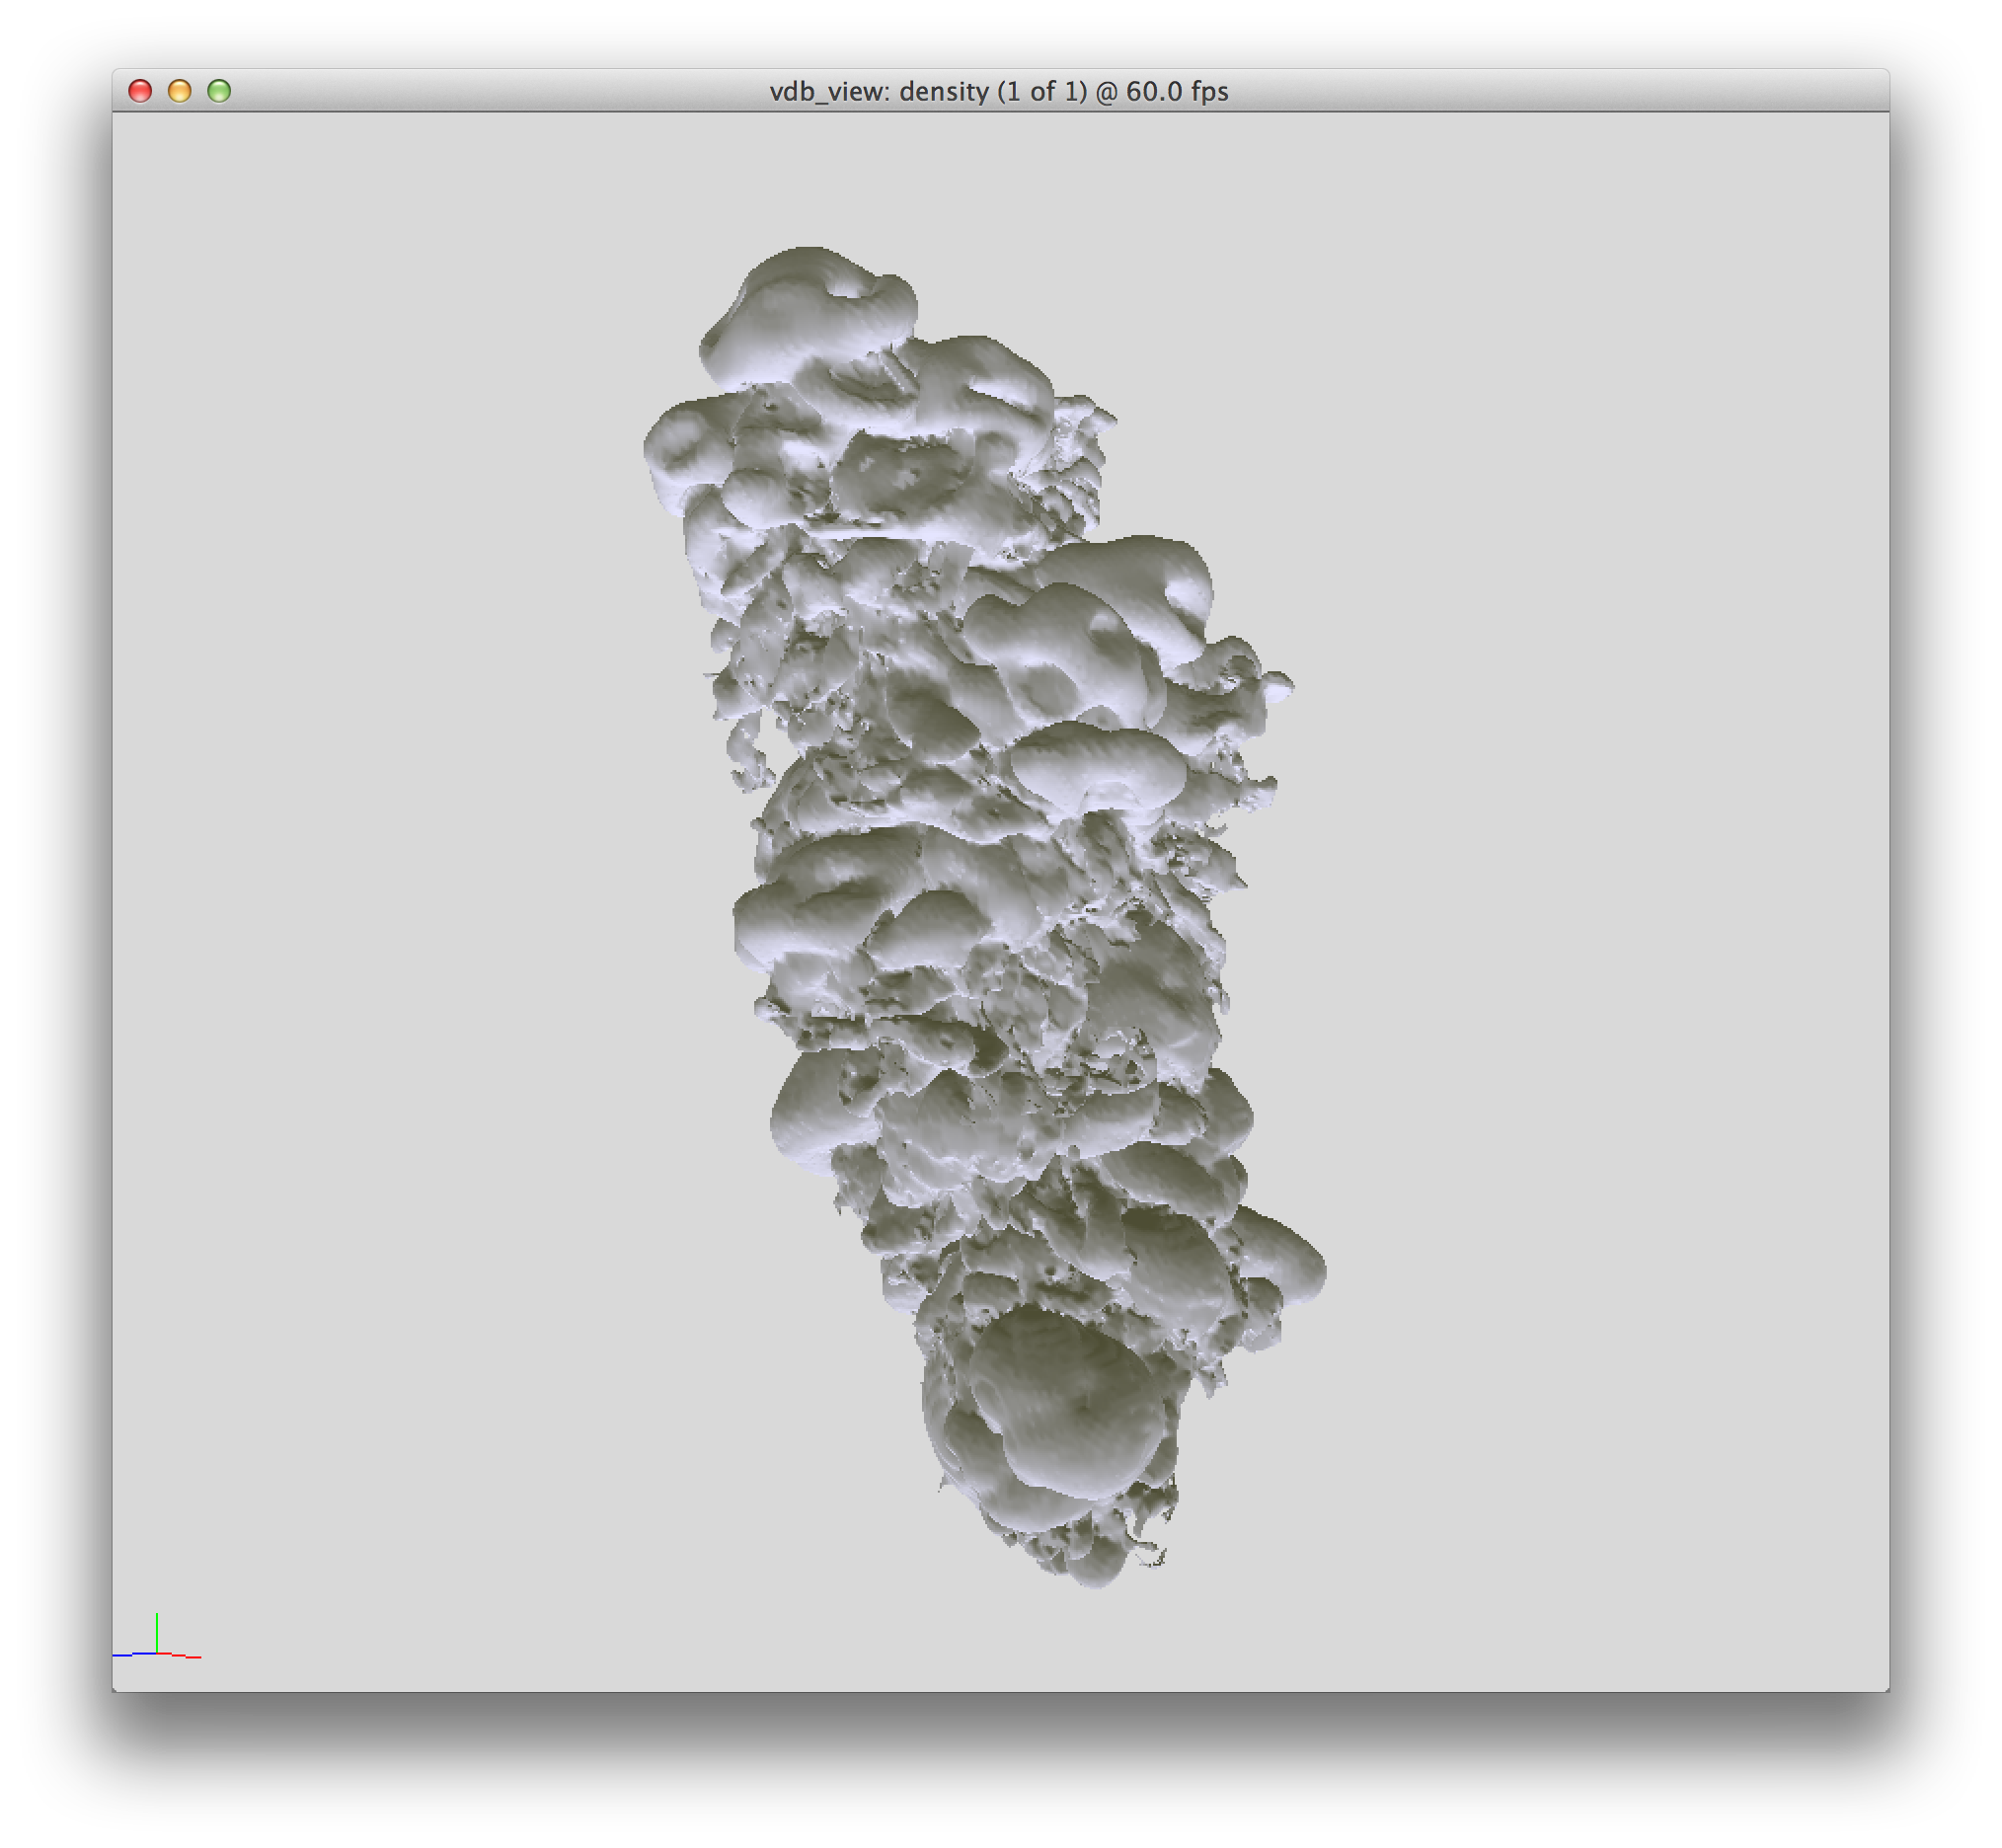
\includegraphics[width=\textwidth]{vdb_view1}
        \end{subfigure}%
        ~ %add desired spacing between images, e. g. ~, \quad, \qquad etc.
          %(or a blank line to force the subfigure onto a new line)
        \begin{subfigure}{0.3\textwidth}
                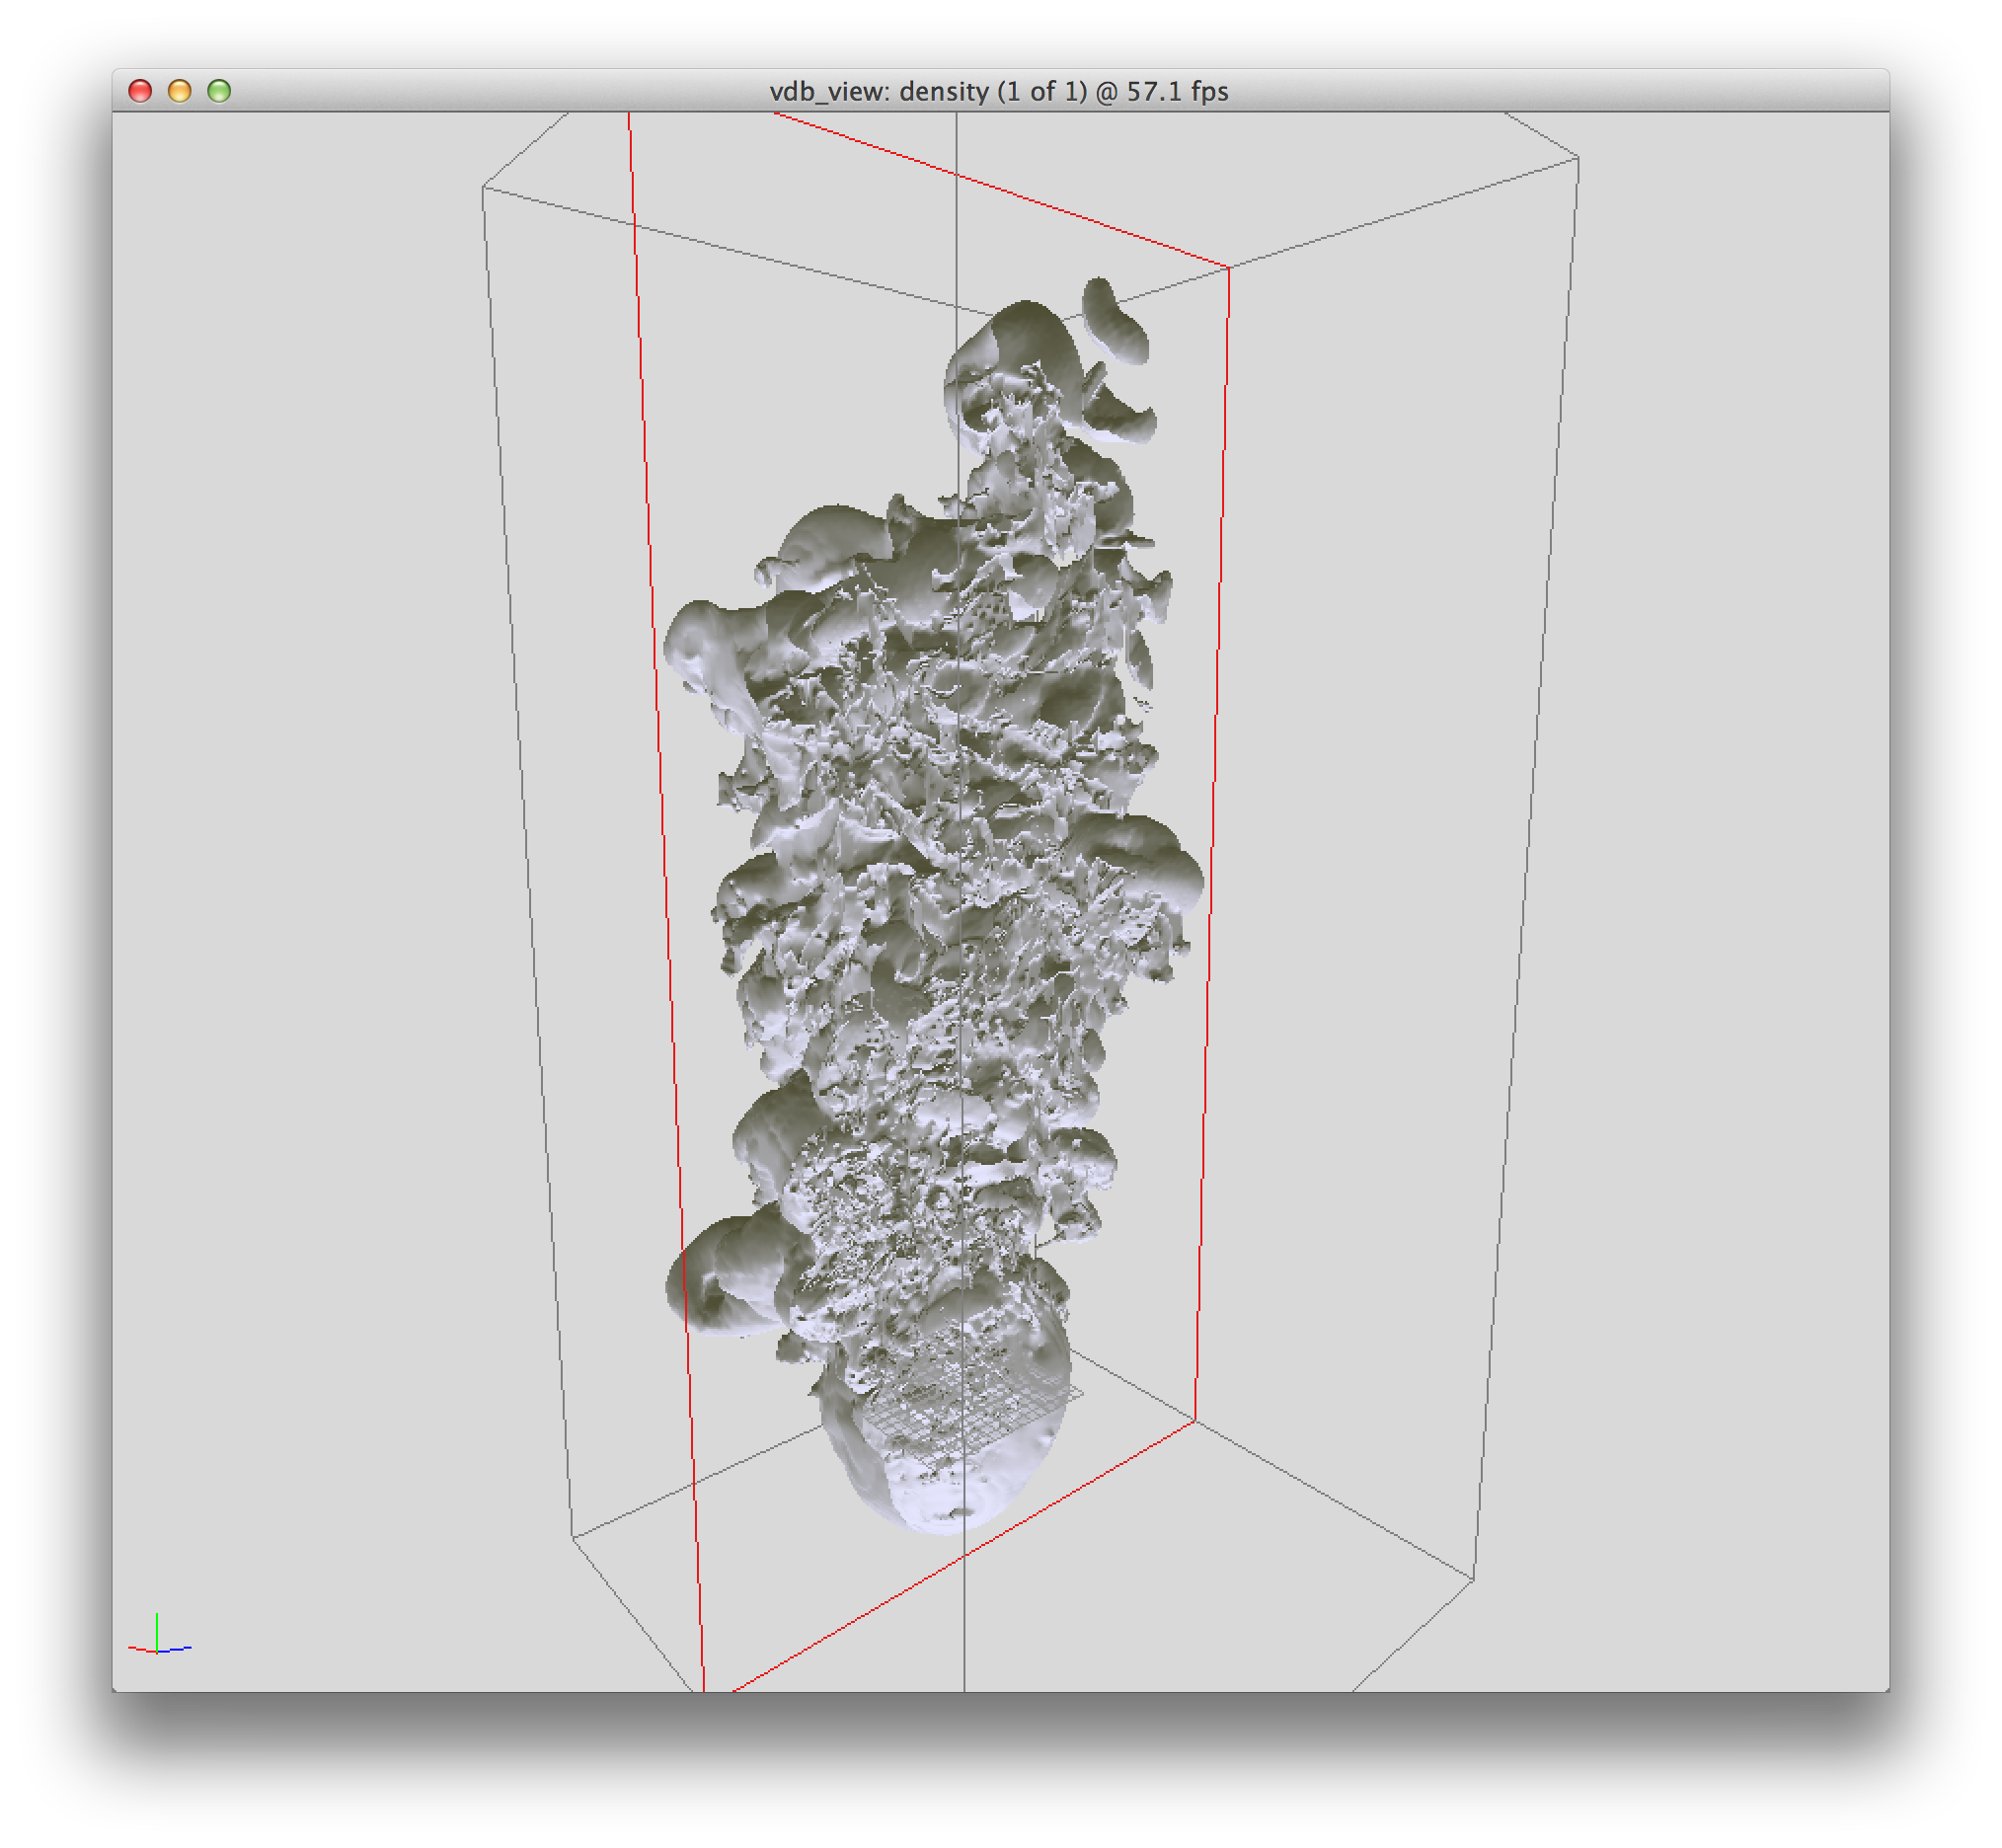
\includegraphics[width=\textwidth]{vdb_view2}
        \end{subfigure}
        ~ %add desired spacing between images, e. g. ~, \quad, \qquad etc.
          %(or a blank line to force the subfigure onto a new line)
        \begin{subfigure}{0.3\textwidth}
                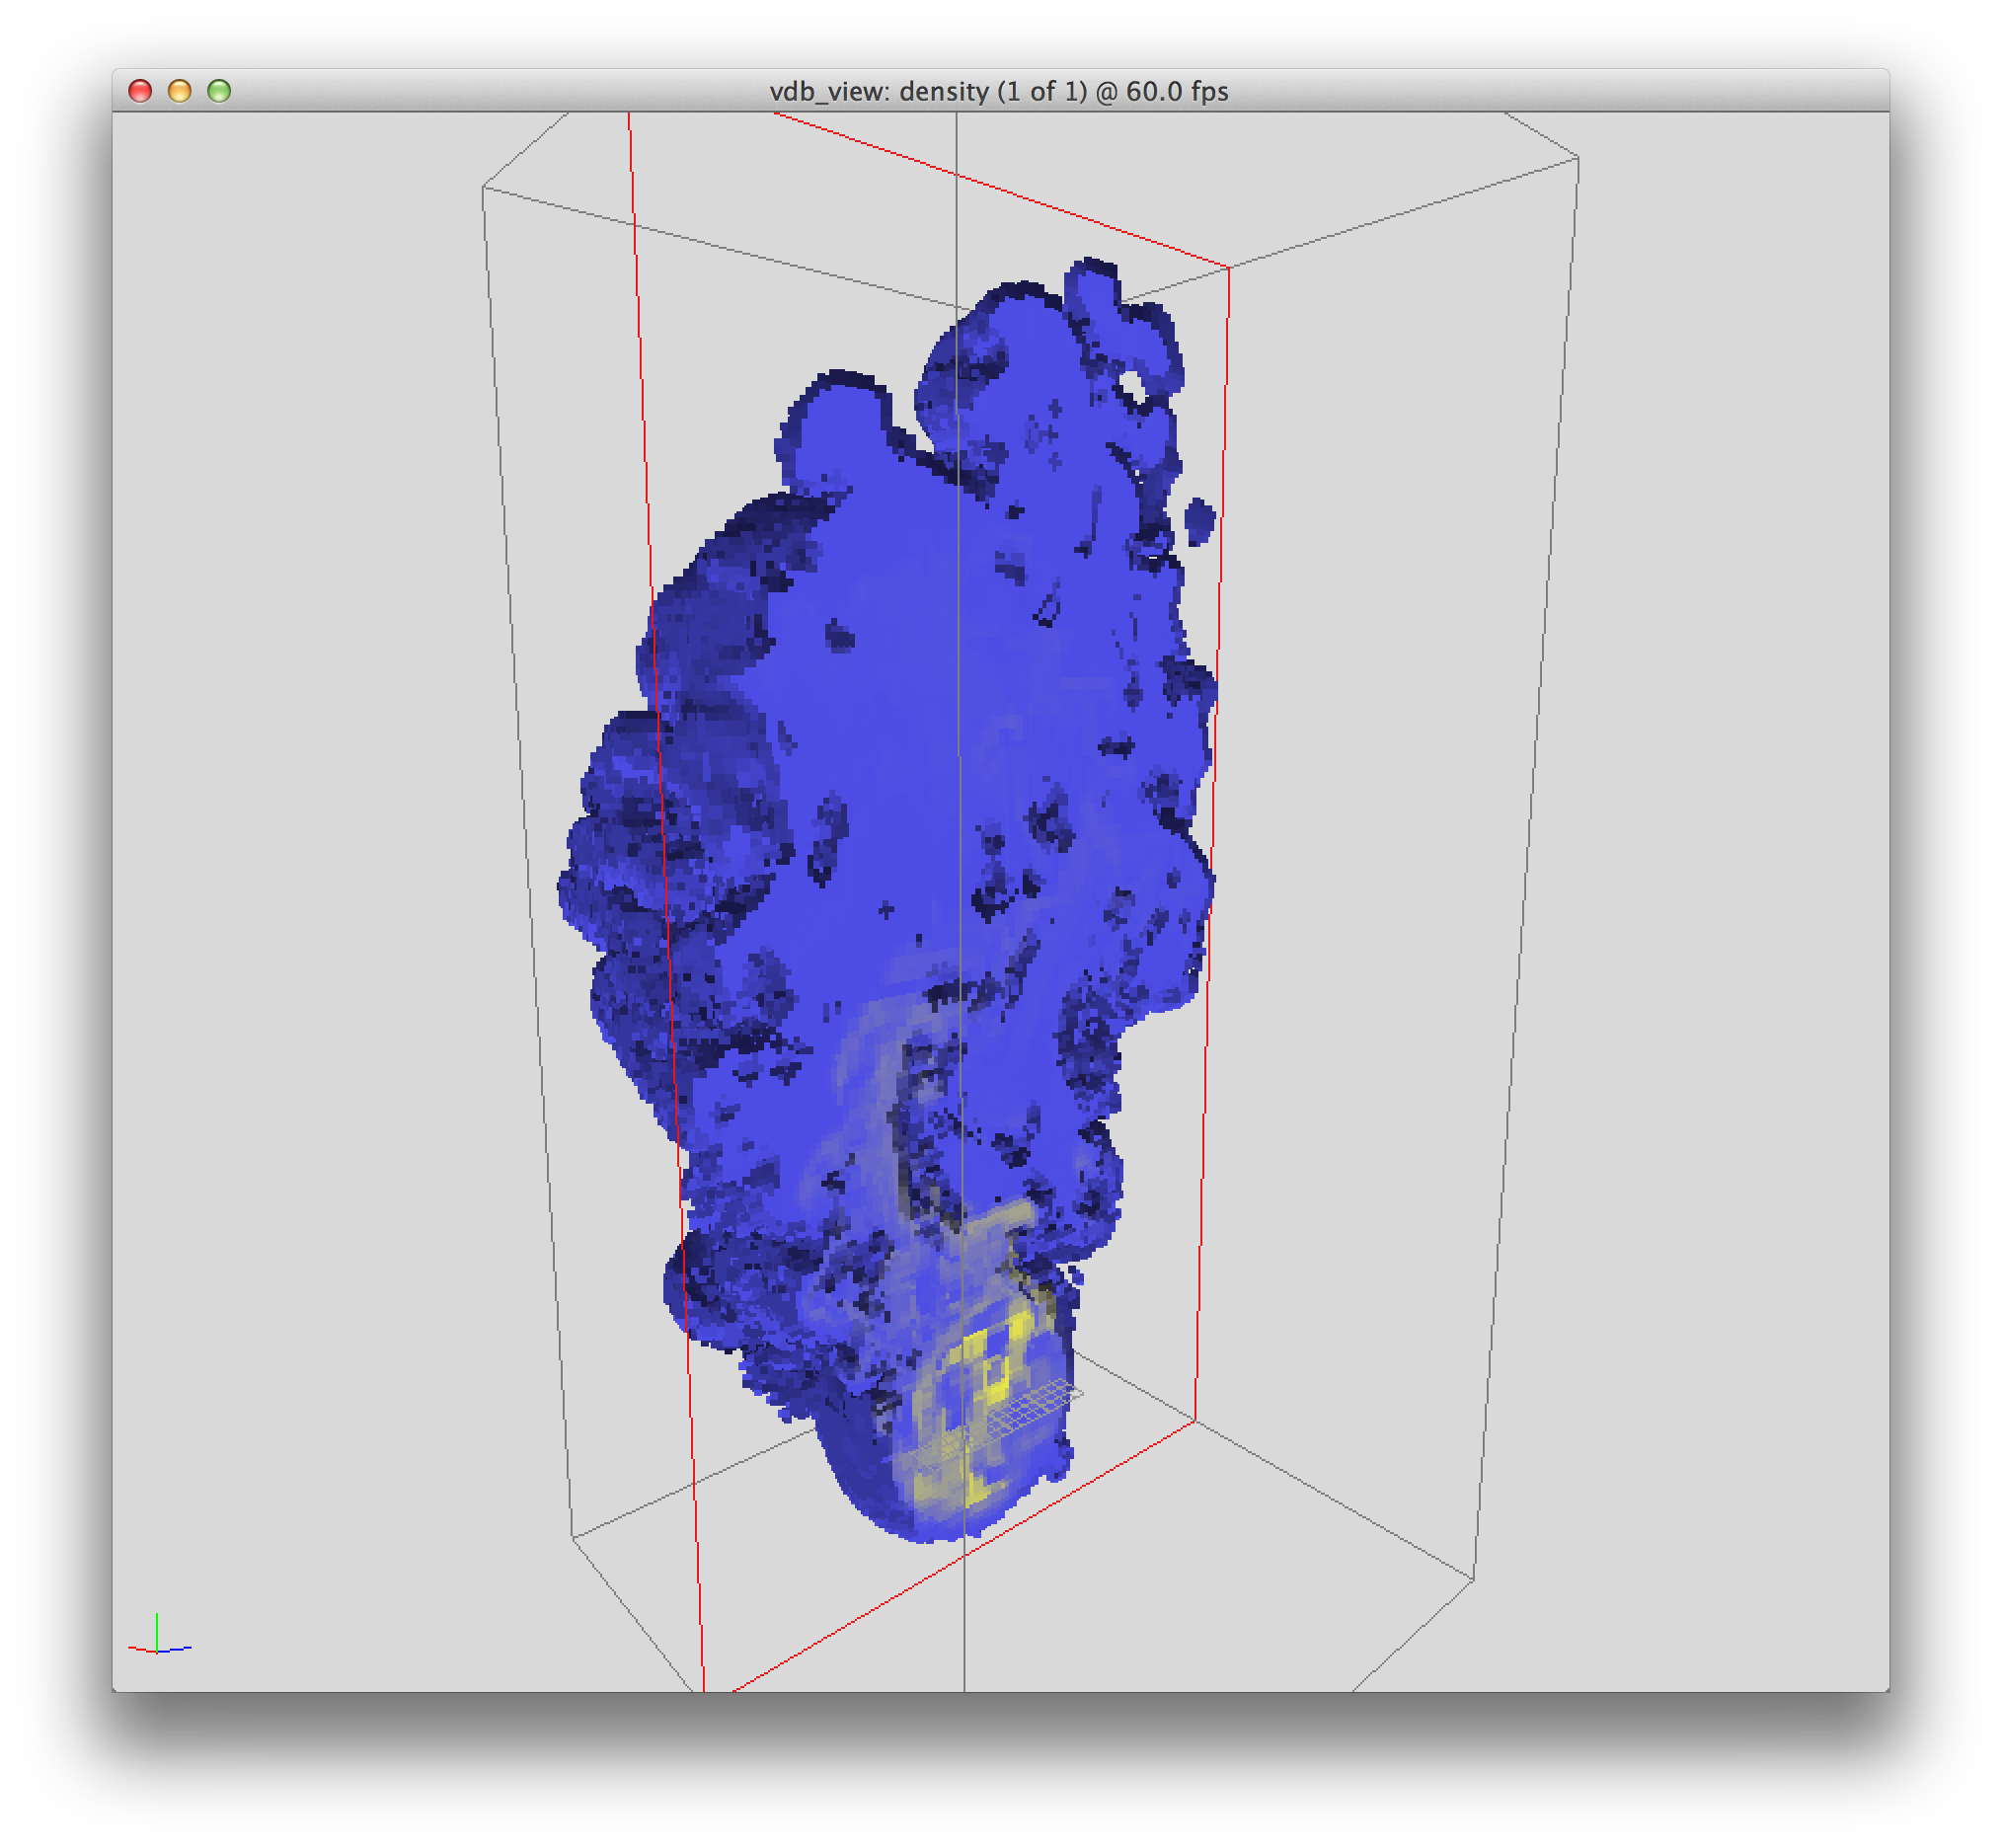
\includegraphics[width=\textwidth]{vdb_view3}
        \end{subfigure}
\end{figure}


\end{frame}
%%%%%%%%%%%%%%%%%%%%%%%%%%%%%%%%%%%%%%%%%%%%%%%%%%%%%%%%%	
\begin{frame}

\frametitle{Tarefas concluídas}

\begin{itemize}
\item Incorporação do código-fonte da biblioteca OpenVDB à solução do Blender
	\begin{itemize}
		\item Problemas de integração
		\item Processo manual
		\item Quebras de compatibilidade e \emph{namespaces}
	\end{itemize}
\item Transformações e Sistemas de Coordenadas
\begin{itemize}
		\item Diferentes espaços: objeto, mundo, volume
\end{itemize}
\item Implementação de técnicas de \emph{wrapping}
	\begin{itemize}
		\item Espelho, por eixo
		\item Truncamento
		\item Periódico
	\end{itemize}
\item Interface para avaliação de volumes por {\it scripts} \emph{OSL}
\end{itemize}

\end{frame}

%%%%%%%%%%%%%

%%%%%%%%%%%%%
%%%%%%% n-th Slide %%%%%%%%%%%%%%%%%%%%%%%%%%%%%%%%%%%%%%%%%

\begin{frame}

\frametitle{Rede de nós para uso de {\it scripts OSL}}

\begin{figure}[!htb]
\center
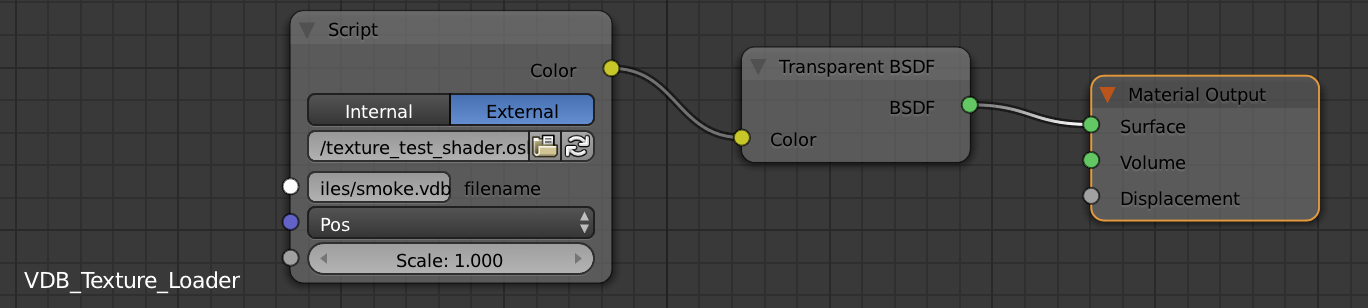
\includegraphics[width=10cm]{vdb_node}
\end{figure}


\end{frame}
%%%%%%%%%%%%%%%%%%%%%%%

%%%%%%%%

\begin{frame}

\frametitle{Exemplo de uso com OSL}

\lstinputlisting[caption={Chamada em OSL para uso da renderização de volumes VDB}]{../sourceCode/tex3d.cpp}

\end{frame}
%%%%%%%%


\begin{frame}

\frametitle{Interface com fatia do volume renderizado}

%figura aqui!! :-P
\begin{figure}[!htb]
\center
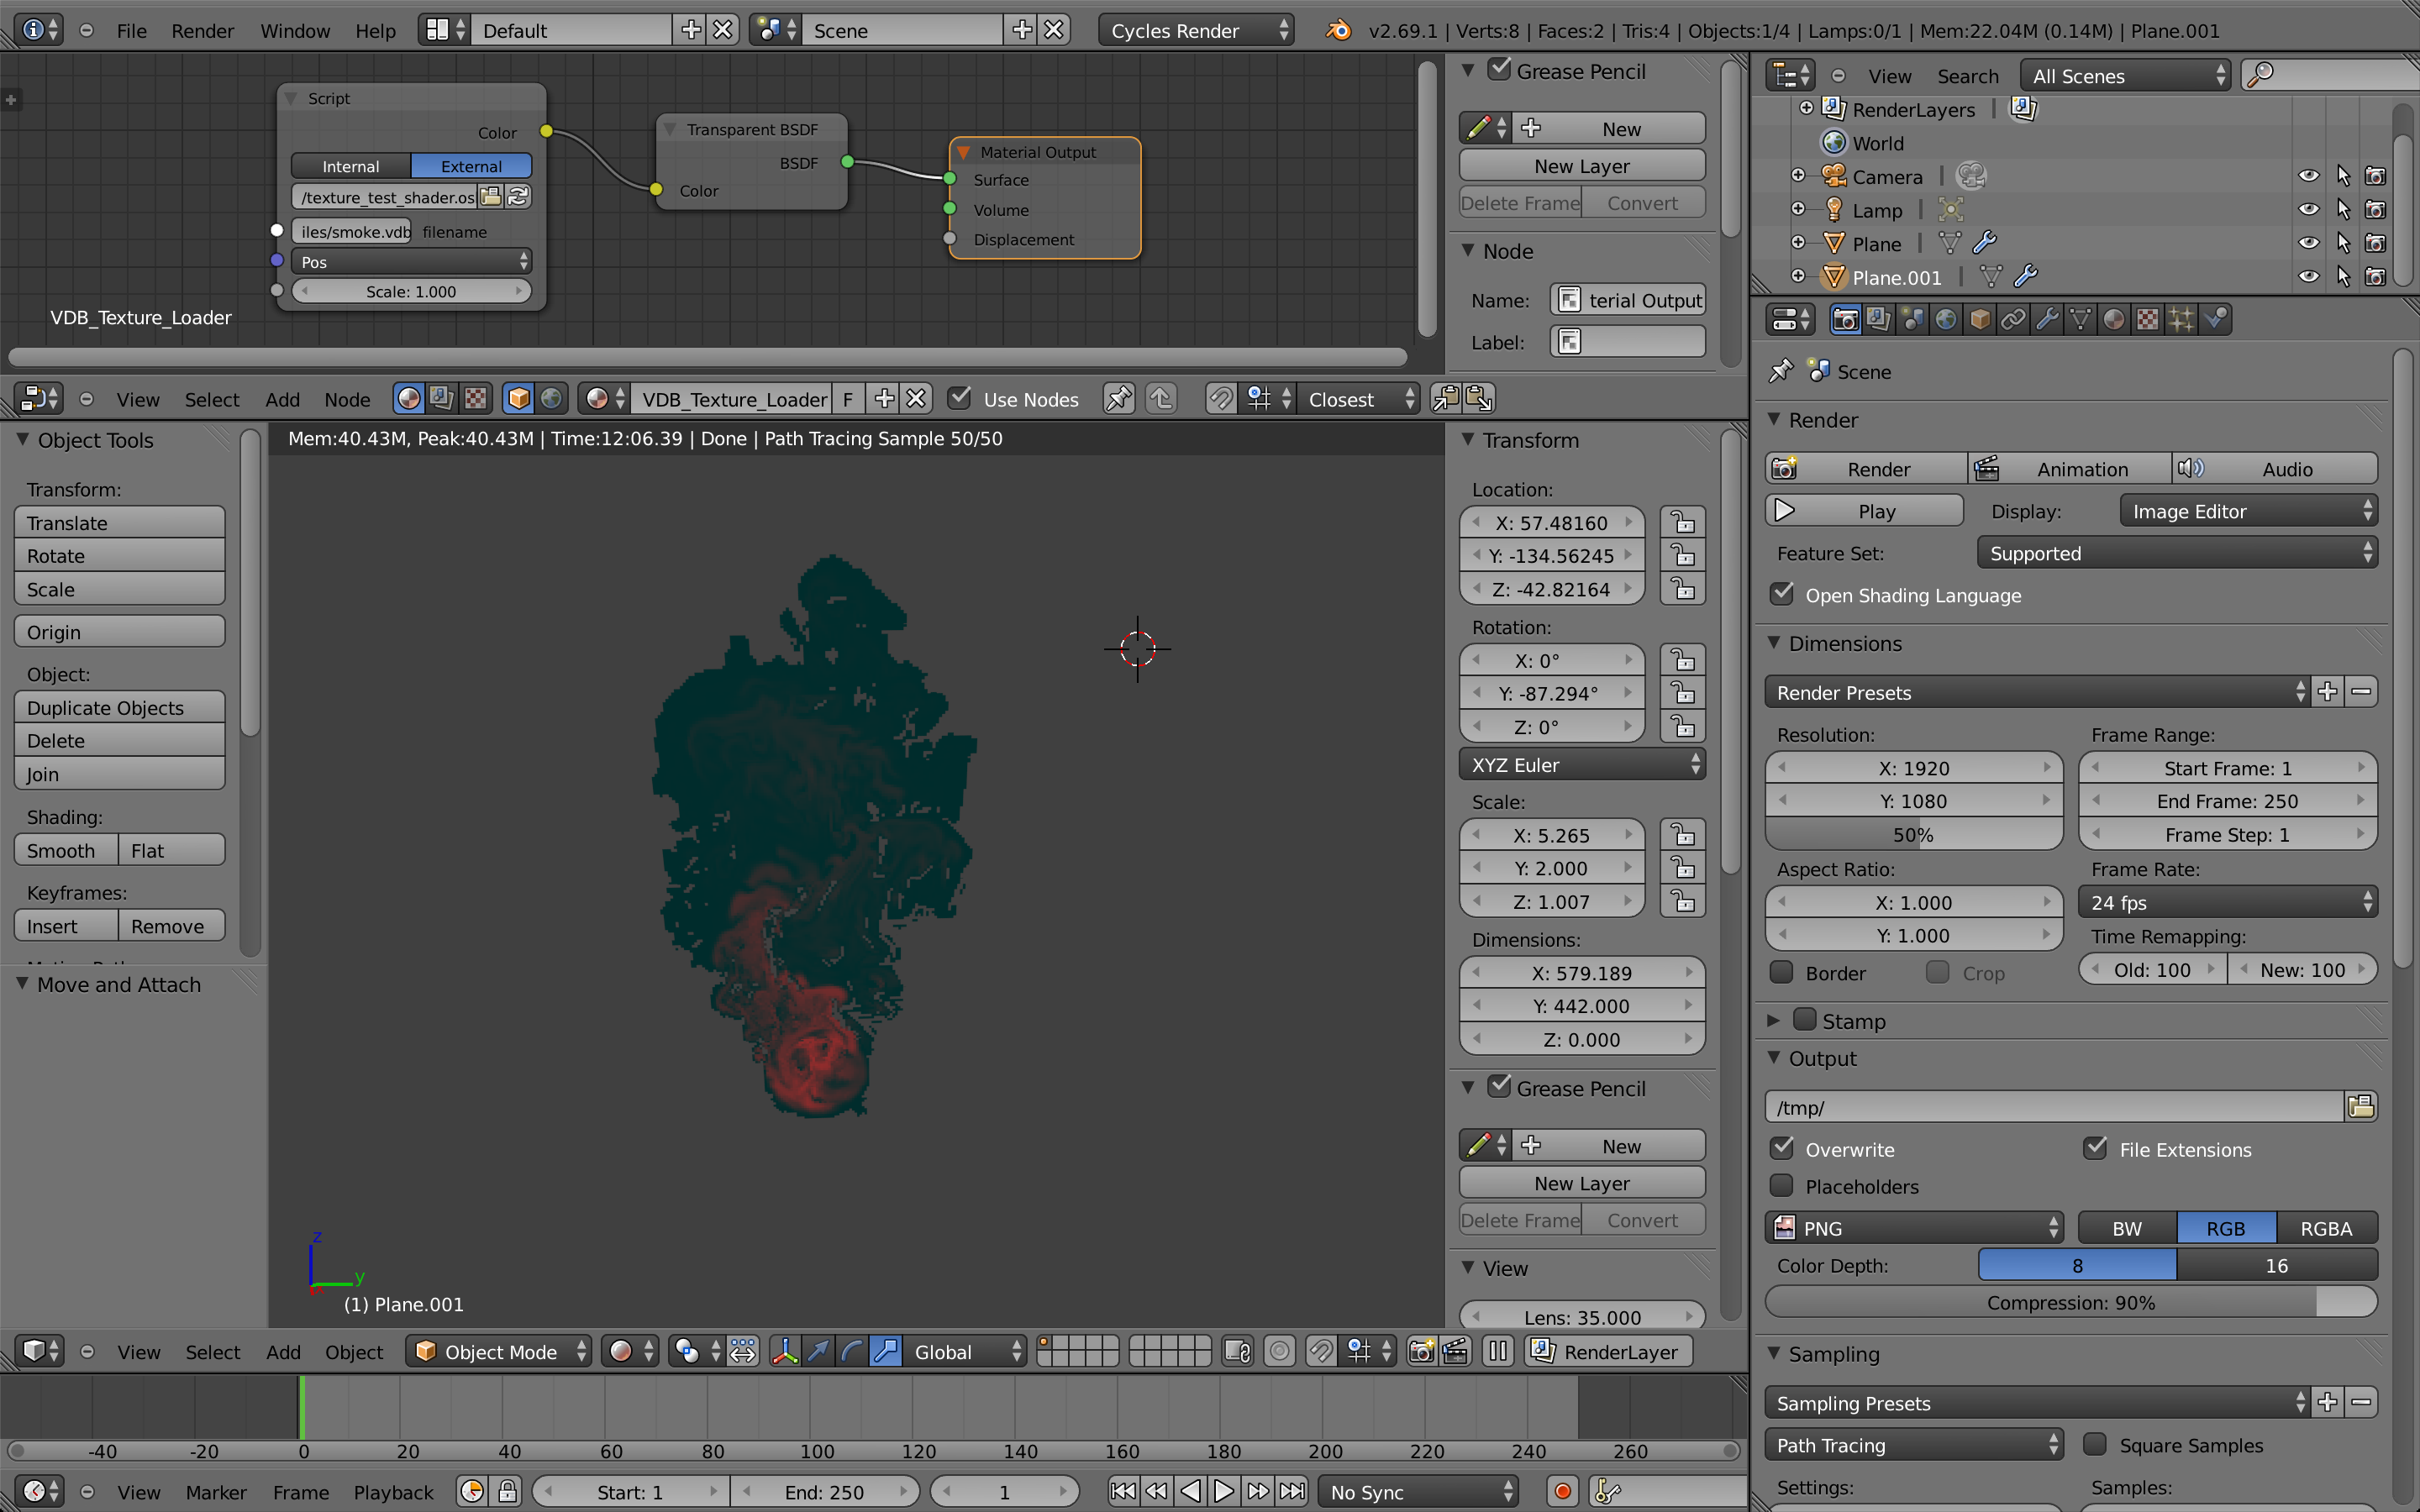
\includegraphics[width=10cm]{vdb_blender_interface}
\end{figure}
\end{frame}
%%%%%%% n-th Slide %%%%%%%%%%%%%%%%%%%%%%%%%%%%%%%%%%%%%%%%%

\begin{frame}

\frametitle{Exemplos de \emph{wrapping}: espelhamento em torno de eixos}

\begin{figure}[!htb]
        \centering
        \begin{subfigure}{0.3\textwidth}
                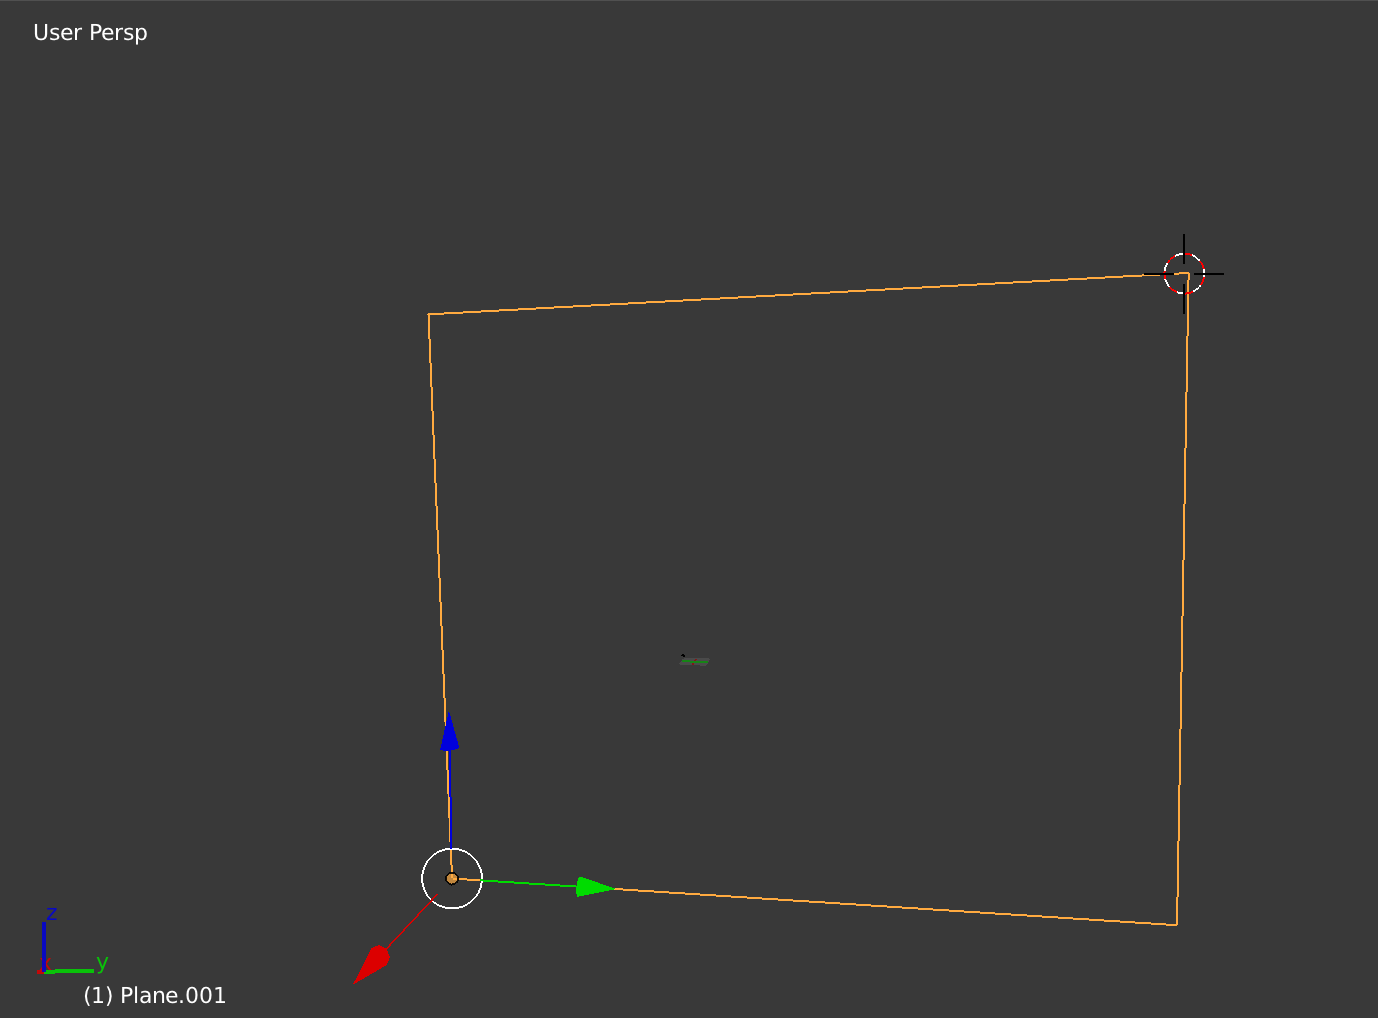
\includegraphics[width=\textwidth]{transf_geometry}
        \end{subfigure}%
        ~ %add desired spacing between images, e. g. ~, \quad, \qquad etc.
          %(or a blank line to force the subfigure onto a new line)
        \begin{subfigure}{0.3\textwidth}
                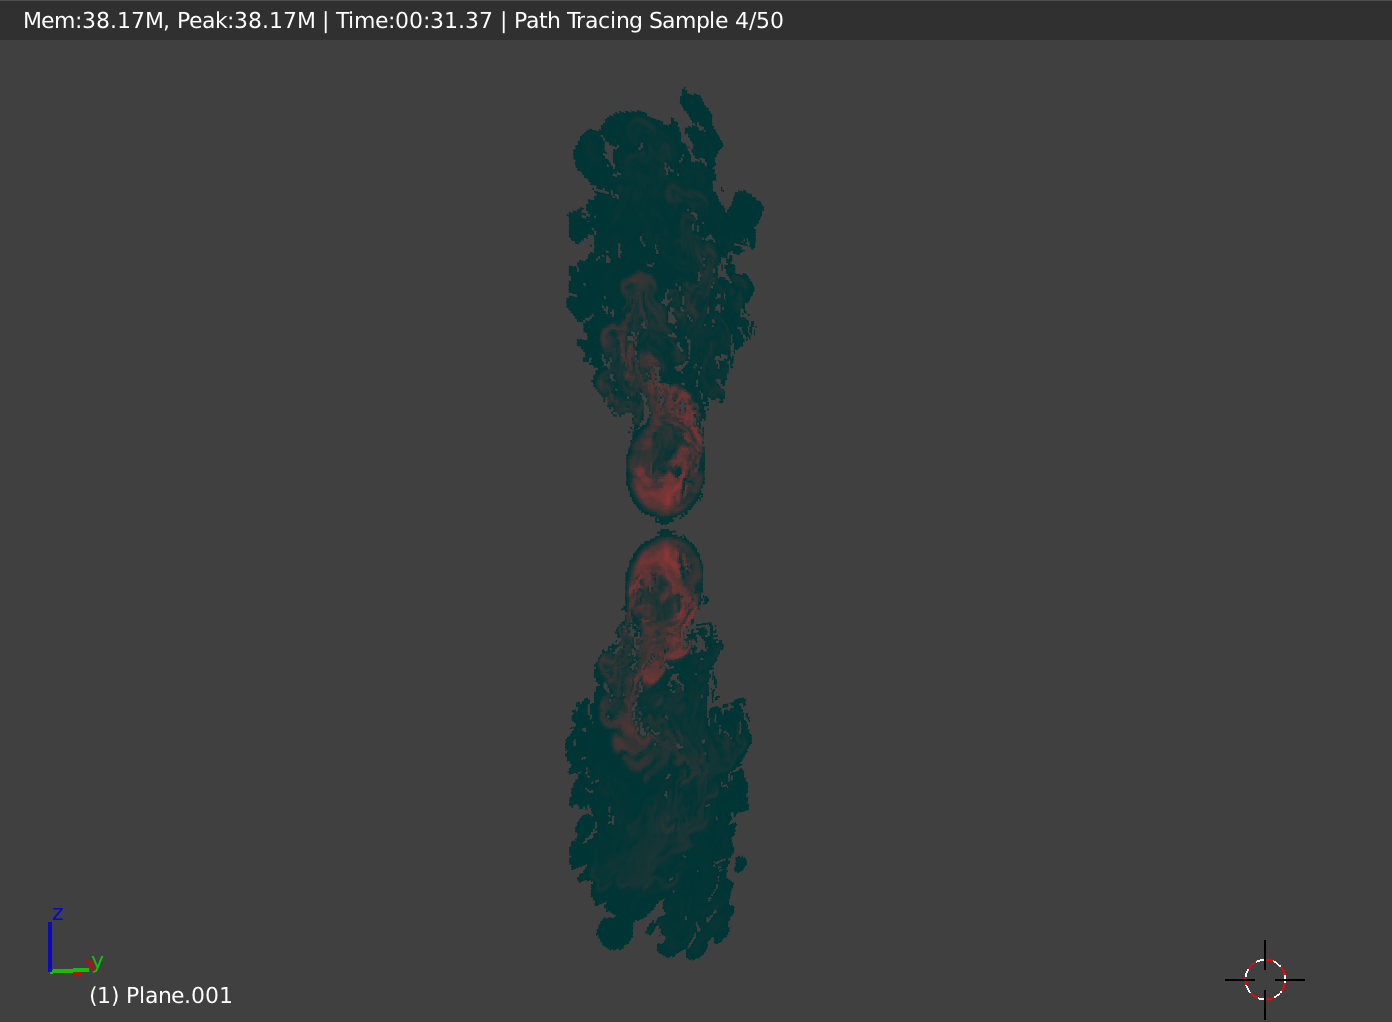
\includegraphics[width=\textwidth]{transf_upsideDown}  
        \end{subfigure}
        ~ %add desired spacing between images, e. g. ~, \quad, \qquad etc.
          %(or a blank line to force the subfigure onto a new line
        \begin{subfigure}{0.3\textwidth}
                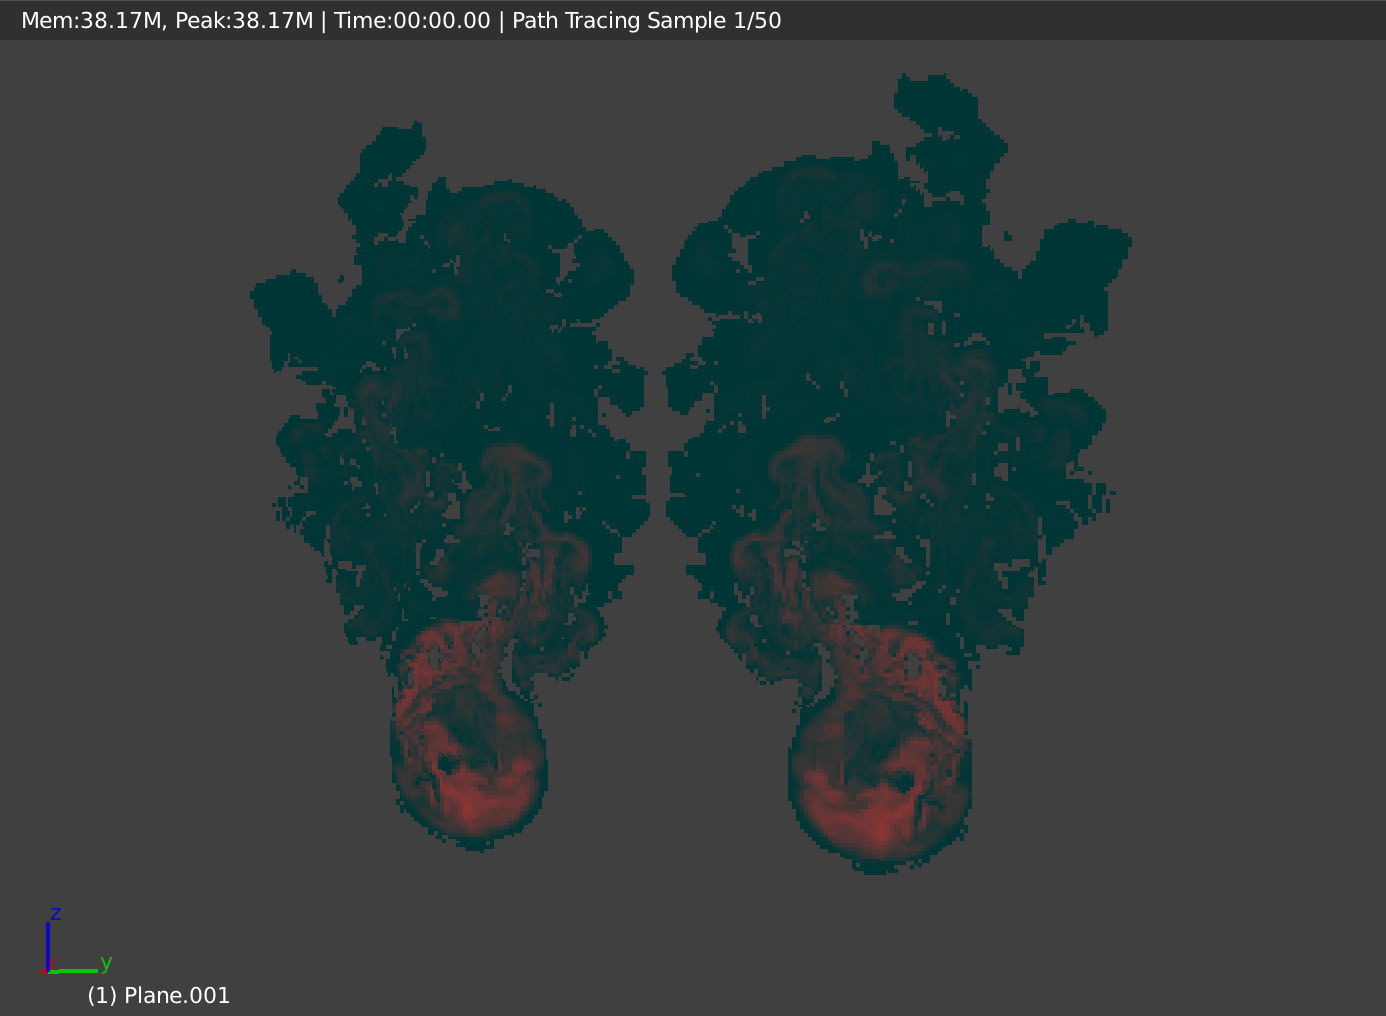
\includegraphics[width=\textwidth]{transf_Mirror}
        \end{subfigure}    
\end{figure}
\end{frame}

%%
\begin{frame}

\frametitle{Uso de memória}
\begin{table}[!ht]
    \centering
    \scalebox{0.8}[1]{
        \begin{tabular}{|c|c|c|}
\hline

\multicolumn{3}{|c|}{\bf{Consumo de memória para representação do volume}} \\
\hline \hline
Estrutura de Dados & Consumo de Memória em {\it bytes} & Valor Relativo\\

\hline
 
Vetores 3D (Estrutura existente) & $10.793.640$ &  $1.545$  \\

\hline
 
OpenVDB & $6.984.656$ & $1$ \\

\hline
 

%\hline
\end{tabular}}
    \caption{Comparação entre o uso de memória da implementação anterior com o uso da estrutura VDB.}
\end{table}
\end{frame}
%%


\section{Conclusão}
\subsection{}
\frametitle{Conclusão}
\begin{frame}
\begin{itemize}
\item Dificuldades e desafios
\begin{itemize}
\item Configuração de código-fonte
\item Vazamentos de memória
\item Transformações e sistemas de coordenadas
\item Sistemas de controle de versionamento  
\end{itemize}
\item Experiência
\end{itemize}


\end{frame}
%%%%%%%%%%%%%%%%%%%%%%%%%%%%%%%%%%%%%%%%%%%%%%%%%%%%%%%%%
\begin{frame}

\frametitle{Trabalhos Futuros}

\begin{itemize}
\item Suporte à execução paralela \\ A biblioteca OpenVDB suporta {\it multi-threading}
\item Criação de interface de usuário \\ Criação de um nó específico para este tipo de volume
\item Permitir que volumes do Blender sejam exportados em {\it VDB} \\ Especialmente para exportar volumes gerados pelo simulador de fumaça do Blender
\end{itemize}

\end{frame}
%%%%%%%%%%%%%%	

\begin{frame}

\centerline{\Huge{Obrigado!}}
\end{frame}

\end{document}